\documentclass[11pt,a4paper]{article}
\usepackage[a4paper,margin=20mm]{geometry}
\usepackage[T1]{fontenc}
\usepackage[utf8]{inputenc}
\usepackage{lmodern,amsmath,amssymb,array,booktabs,longtable,pdflscape,graphicx}
\usepackage[table]{xcolor}
\usepackage{titlesec}
\usepackage[expansion=false]{microtype}
\usepackage{cite}
\usepackage{xurl}
\usepackage[font=small,labelfont=bf]{caption}
\usepackage[hidelinks]{hyperref}
\urlstyle{same}
\graphicspath{{../../research_figures/}{research_figures/}}
\definecolor{headgray}{HTML}{E8EDF2}
\definecolor{titleblue}{HTML}{243D59}
\newcolumntype{L}[1]{>{\raggedright\arraybackslash}p{#1}}
\newcommand{\ind}{\mathbf{1}}
\newcommand{\A}{\textbf{A:}\ }
\newcommand{\R}{\textbf{R:}\ }
\setlength{\parindent}{0pt}
\setlength{\parskip}{5pt}
\setlength{\tabcolsep}{3pt}
\setlength{\emergencystretch}{3em}
\setlength{\LTpre}{6pt}
\setlength{\LTpost}{6pt}
\setlength{\LTcapwidth}{\textwidth}
\renewcommand{\arraystretch}{1.12}
\titlespacing*{\section}{0pt}{12pt}{6pt}
\titlespacing*{\subsection}{0pt}{9pt}{4pt}
\setlength{\textfloatsep}{12pt plus 2pt minus 2pt}
\setlength{\intextsep}{10pt plus 2pt minus 2pt}
\clubpenalty=10000
\widowpenalty=10000
\displaywidowpenalty=10000
\raggedbottom
\hypersetup{pdftitle={Phase 2: Evidence Reliability in Explainable Data Drift Monitoring},pdfauthor={Ahmed Bilal (23I-2581) and Umer Behram (23I-2604)}}

% Phase 2 research proposal. Word files and implementation code are unchanged.
\begin{document}
\begin{titlepage}
\centering
\vspace*{20mm}
{\large Data Analysis and Visualization\par}
\vspace{3mm}
{\normalsize Phase 2 Research Proposal\par}
\vspace{20mm}
\begin{minipage}{0.85\textwidth}
\centering
{\color{titleblue}\LARGE\bfseries
Evidence Reliability in Explainable Data Drift Monitoring\par}
\vspace{7mm}
{\large Extended Literature Review and\par
Research Methodology Development\par}
\end{minipage}
\vspace{14mm}
{\color{titleblue}\rule{0.56\textwidth}{0.5pt}\par}
\vspace{11mm}
{\large Ahmed Bilal\par}
{\normalsize 23I-2581\par}
\vspace{6mm}
{\large Umer Behram\par}
{\normalsize 23I-2604\par}
\vfill
{\normalsize 6 November 2026\par}
\vspace*{14mm}
\end{titlepage}
\pagestyle{plain}
\setcounter{page}{1}

\subsection*{Continuity with Phase 1 and Scope Refinement}
Phase 1 motivated connecting drift detection, feature-level explanation and
predictive consequences. This proposal narrows that direction to frozen
tabular classifiers, so monitoring evidence can be evaluated without confounding
it with model updates. The study will distinguish input change from material
excess classification error, account for delayed labels and specify a
cohort-aligned display. This submission specifies proposed work; it reports no
completed implementation or measured project results. Here, explainability
means transparent cohort-level evidence and marginal feature screening; it
does not mean identified causal root causes. Image-domain transfer, adaptive intervention and analyst
decision benefit require subsequent studies \cite{greco,szucs,guerrero,driftvis,souza}.

\section*{Deliverable 1 --- Extended Literature Review}
\subsection*{Additional Paper Selection}
The extended corpus comprises ten original 2025--2026 conference papers or
research chapters absent from the retained Phase 1 bibliography. Bibliographic years follow the
publisher's recommended published-volume citation, with earlier online dates
noted separately where relevant; a conference-event or preprint date is not
substituted for publication. These selections use the brief's conference-paper and book-chapter
eligibility routes; no journal-quartile claim is made for them. Each full text
was assessed for relevance and identifiable data, methodology and evaluation.
This is a focused corpus review, not an exhaustive systematic review. Older
foundations, dataset provenance and operational guidance remain supporting references outside the
ten-paper count \cite{cerqueira,window,pudd,batched,causal,prodem,conformal,timans,pprm,suitability}.

For each selection, the review records publication metadata, the full-text
version examined, data and label access, preprocessing, comparison methods,
evaluation target and limitations. Table~\ref{tab:comparison} compares all ten
studies under the same headings. S2, S6, S9 and S10 anchor the gap matrix
through reference-window meaning, delayed-label error prediction, sequential
predictive risk and margin-based suitability. The remaining studies supply
benchmarking, label-access, explanation and bounded-risk context. This focused
selection is based on methodological relevance; these four anchors do not
represent the entire field \cite{window,prodem,pprm,suitability}.

The focused follow-up through 6 November used publisher and author-archive searches for risk
monitoring, harmful distribution shifts, accuracy degradation and suitability,
followed by citation checking and full-text screening. S6 and S8--S10 strengthen
coverage of explicit risk and decision targets. The follow-up search log records the actual
queries, retrieval date, source versions and selection decisions.

\subsection*{Paper-Selection Eligibility Audit}
The selected-paper set is exactly S1--S10, rather than the entire reference
list. Publication year, title, venue and research-paper status were checked
against publisher records and reviewed full-text versions through
6 November 2026, including the closer risk/suitability studies S6 and S8--S10.
The extension was checked
against the retained Phase 1 bibliography to avoid counting a paper twice.
Matching that retained version to the final submitted Phase 1 bibliography
remains a document-provenance check before additionality can be finalized.
The reviewed full texts provide the data, method and evaluation evidence
summarized below and critically compared in Table~\ref{tab:comparison}.
All ten are original research contributions published in conference
proceedings, including proceedings chapters; none is an editorial, opinion
piece, news item or general webpage. They therefore use the supplied
requirement's conference-paper or book-chapter route. No journal Q1--Q2
classification is asserted for these proceedings.

\begingroup
\small
\begin{longtable}{L{0.8cm}L{1.4cm}L{4.5cm}L{9.0cm}}
\caption{Eligibility of the ten selected papers under the supplied selection requirements.}\label{tab:eligibility}\\
\toprule\rowcolor{headgray}
\textbf{Study}&\textbf{Year}&\textbf{Published route / publisher}&\textbf{Relevant research and assessable evidence}\\\midrule\endfirsthead
\toprule\rowcolor{headgray}
\textbf{Study}&\textbf{Year}&\textbf{Published route / publisher}&\textbf{Relevant research and assessable evidence}\\\midrule\endhead
\midrule\multicolumn{4}{r}{\emph{Continued on next page}}\\\endfoot
\bottomrule\endlastfoot
S1 \cite{cerqueira} & 2026 & KDD conference paper; ACM. & Detector evaluation: seven datasets, controlled drift injection, multiple detectors and timing-aware detection metrics.\\[3pt]
S2 \cite{window} & 2026 & IDA conference paper / LNCS chapter; Springer. & Reference-window interpretation: analytical example and eleven-stream comparisons of detection, learning and reset strategies.\\[3pt]
S3 \cite{pudd} & 2025 & AAAI technical-track conference paper; AAAI Press. & Label-dependent monitoring: PU-index derivation, adaptive bucketing and structured/image-stream evaluations with accuracy and ranks.\\[3pt]
S4 \cite{batched} & 2025 & ICDM Workshops research paper; IEEE. & Label-free monitoring: Gaussian mean, variance and covariance simulations; batched distances, error rates and computational-budget comparisons.\\[3pt]
S5 \cite{causal} & 2026 & ECML PKDD workshop proceedings chapter; Springer CCIS. & Drift explanation: semi-synthetic Adult/Student data, causal discovery and repeated graph/feature-recovery evaluations.\\[3pt]
S6 \cite{prodem} & 2026\newline online 2025 & ECML PKDD applied-data-science conference paper / LNAI chapter; Springer. & Frozen-model degradation under delayed labels: two proprietary fraud datasets, learned error prediction, instance-error metrics and monthly alerts.\\[3pt]
S7 \cite{conformal} & 2025 & COPA conference paper; PMLR. & Recurrence and label access: STAGGER, Electricity and Airlines; conformal martingales, model reuse and accuracy/training-cost evaluation.\\[3pt]
S8 \cite{timans} & 2025 & UAI conference paper; PMLR. & Bounded-risk monitoring: betting processes, outlier/set-prediction tasks, false-alarm control and repeated delay comparisons.\\[3pt]
S9 \cite{pprm} & 2026 & ICML conference paper; PMLR. & Predictive-risk monitoring: image, language-model and communications tasks; prediction-powered estimates, confidence sequences and alarm-time comparisons.\\[3pt]
S10 \cite{suitability} & 2025 & ICML conference paper; PMLR. & Accuracy-margin decisions: three WILDS datasets, correctness estimation, non-inferiority testing and suitability-decision evaluation.\\
\end{longtable}
\endgroup

\textbf{Date and venue distinctions.} S5 was published in 2026 despite the
2025 workshop-event name. S6 follows Springer's recommended 2026 volume
citation; its first-online date is 29 September 2025, so both dates fall within
the permitted period. S4 and S5 are explicitly identified as workshop
proceedings research, rather than main-track papers. Eligibility rests on
their published research-paper/chapter status, not an invented journal rank
\cite{causal,prodem,batched}.

\textbf{Sources outside the selected-paper count.} Earlier research,
statistical foundations, standards and operational documentation are cited
only where needed to attribute methods or qualify the research gap. The
brief's 8--10 eligible additional selections are the ten studies S1--S10;
supporting sources do not contribute to that count. In particular, the 2022
ICLR risk-monitoring paper is supporting prior work, and
the 2026 evidence-sufficiency preprint is not a published proceedings or
journal selection. A publication's inclusion in the reference list must not
be interpreted as a claim that it belongs to S1--S10.

\begin{landscape}
\subsection*{Cross-Paper Comparison of All Ten Selected Studies}
\small
Table~\ref{tab:comparison} compares the complete additional corpus using the
same nine headings. Venue information appears beneath each title.
\textbf{A} identifies an author-stated limitation or assumption;
\textbf{R} identifies this review's methodological inference. Results remain
attached to their original tasks and comparators; they are not a common
performance ranking. S6 follows Springer's 2026 volume citation and was first
published online in 2025.
Section, equation and table locators refer to the reviewed full-text versions
identified in the source register; publication records establish eligibility.

\begingroup
\fontsize{9.2}{11.2}\selectfont
\setlength{\tabcolsep}{3pt}
\setlength{\LTcapwidth}{\linewidth}
\renewcommand{\arraystretch}{1.08}
\begin{longtable}{L{0.65cm}L{4.0cm}L{0.85cm}L{2.9cm}L{2.8cm}L{2.8cm}L{2.4cm}L{3.0cm}L{4.2cm}}
\caption{Cross-paper comparison of all ten additional research studies (S1--S10).}\label{tab:comparison}\\
\toprule\rowcolor{headgray}
\textbf{ID}&\textbf{Paper title and venue}&\textbf{Year}&\textbf{Dataset used}&\textbf{Preprocessing}&\textbf{Models / techniques}&\textbf{Evaluation metrics}&\textbf{Reported results}&\textbf{Limitations / research gap}\\
\midrule\endfirsthead
\multicolumn{9}{l}{\small\emph{Table \thetable\ continued: comparison of the ten selected studies}}\\[3pt]
\toprule\rowcolor{headgray}
\textbf{ID}&\textbf{Paper title and venue}&\textbf{Year}&\textbf{Dataset used}&\textbf{Preprocessing}&\textbf{Models / techniques}&\textbf{Evaluation metrics}&\textbf{Reported results}&\textbf{Limitations / research gap}\\
\midrule\endhead
\midrule\multicolumn{9}{r}{\emph{Continued on next page}}\\\endfoot
\bottomrule\endlastfoot
\textbf{S1} &
A Framework for Evaluating and Benchmarking Concept Drift Detection Methods \cite{cerqueira}.
\par\emph{ACM KDD.} &
2026 &
Asfault, Electricity, Covertype, GasSensorArray, NOAA, Posture and Rialto. &
Shuffle streams; inject class-prior, label-swap, permutation or filtering changes; construct abrupt/gradual transitions. &
Reported fourteen-method benchmark; Hoeffding-tree core; 50 trials per dataset/type; held-out-dataset tuning. &
Event precision, recall, F1; normalized delay; alarm/false-alarm rates; runtime. &
For abrupt class swap, SEED and STEPD have mean ranks 1.1 and 2.4; lower is better. Ranks vary by mechanism (Table~1). &
\A Immediate feedback; removed temporal structure. A restricted five-classifier check supplements the core (Table~12).
\R Event recovery does not establish delayed excess-risk verdict correctness.\\
\addlinespace[5pt]
\textbf{S2} &
The Window Dilemma: Why Concept Drift Detection is Ill-Posed \cite{window}.
\par\emph{IDA; Springer LNCS.} &
2026 &
Eleven binary/multiclass streams, including Electricity, Covertype, Insects, NOAA and Rialto. &
Ordered prequential evaluation; explicit training, window and reset schedules; warm/cold-start analysis. &
DDM, ADWIN, D3, IBDD; NB/trees; adaptive, incremental, resetting and static forests. &
Mean accuracy; kappa; median algorithm rank. &
ARF median rank 2; AMF and incremental RF rank 3; resetting RF rank 4 (Table~1). &
\A Windows need not represent endpoint concepts; natural changes cannot all be verified.
\R Learning-policy comparisons, including delayed schedules, do not isolate frozen-model harm verdicts.\\
\addlinespace[5pt]
\textbf{S3} &
Early Concept Drift Detection via Prediction Uncertainty \cite{pudd}.
\par\emph{AAAI.} &
2025 &
Airline, Electricity, PowerSupply; Sine, Mixed, SEA variants; CIFAR-10-CD. &
True-class scores; separate correct/misclassified instances before adaptive bucketing; window cuts; Markov class-interest image simulation. &
PUDD; chi-square testing; DNN, GNB and VFDT; classic/adaptive baselines. &
Prediction accuracy; average ranks; threshold and bucketing sensitivity. &
First in 17/24 incremental classic-detector comparisons and top three in 20/24 (Experiments). &
\A Manual thresholds and window-pair guarantees.
\R Both true-class scores and correctness-aware bucketing require labels; early sensitivity is not certification of material excess risk.\\
\addlinespace[5pt]
\textbf{S4} &
Flexible and Efficient Drift Detection Without Labels \cite{batched}.
\par\emph{IEEE ICDM Workshops.} &
2025 &
Gaussian simulations with mean, variance and covariance changes; high-dimensional null/shift settings. &
Generate training, reference and detection sets; partition them into equal-size batches and matched triplets. &
Batched distances, including MMD; paired-distance t-tests; computational-budget comparisons. &
False-positive and false-negative rates; detection power; runtime. &
Batching improves power in selected tested time budgets; behaviour depends on distance and shift type (Sec.~III). &
\A Independent batch differences; normality or a large-batch-count approximation. Algorithm~1 uses equal-size sets, with an unequal-size extension discussed.
\R Power against input change does not establish classifier harm.\\
\addlinespace[5pt]
\textbf{S5} &
Causal Explanation of Concept Drift---A Truly Actionable Approach \cite{causal}.
\par\emph{ECML PKDD workshop proceedings; Springer CCIS.} &
2026 &
Semi-synthetic Adult and Portuguese Student Performance drift scenarios. &
Learn and modify Bayesian-network conditional distributions; concatenate pre/post samples; include a time variable. &
PC causal discovery with g-square testing; time-augmented causal explanation. &
Graph orientation and changed-feature identification across ten runs per scenario. &
Occupation is linked to time in 9/10 Adult Women in STEM runs (Secs.~6--7). &
\A A single global causal graph may not represent all subgroups; causal-discovery assumptions are required.
\R Marginal screening in this proposal is a weaker explanation object.\\
\addlinespace[5pt]
\textbf{S6} &
Proactive Detection of Model Degradation in Financial Fraud Prediction with Delayed Labels \cite{prodem}.
\par\emph{ECML PKDD; Springer LNAI.} &
2026 &
Two proprietary payment-network datasets: transaction fraud ($>3$ million/month) and account fraud (about 5 million/month), each spanning nine months. &
Months 1--2 train the primary model; month 3 trains the meta-model; months 4--9 evaluate, relabelled 1--6 in results. &
Frozen XGBoost primary model; FT-Transformer error meta-model; reverse distillation, focal-loss training and heuristic alert thresholds. &
Instance-error precision/recall; first alert month; value detection rate; reported FAR ratio $FP/TP$, distinct from $FP/(FP+TN)$. &
Error precision/recall: 0.66/0.64 (transactions), 0.68/0.65 (accounts). Alerts in evaluation month 4 versus best-baseline month 5 (Tables~1--2, reviewed author version). &
\R Proprietary data and fixed baseline thresholds limit reproducibility/comparison. In the reviewed author version, Eq.~17's estimated value-detection rate still uses true fraud labels in its denominator, requiring clarification for label-free use. No cohort-risk interval guarantee is supplied.\\
\addlinespace[5pt]
\textbf{S7} &
A Conformal Martingales Approach for Recurrent Concept Drift \cite{conformal}.
\par\emph{COPA; PMLR.} &
2025 &
STAGGER, Electricity and Airlines. &
Construct recurrent STAGGER regimes with 0/10\% label noise; form sequential training/calibration and recent-data windows. &
40-tree TreeBagger; inductive conformal martingales; model pool; exchangeability checks and F1-based reuse selection. &
Accuracy; detection delay; false alarms; model-training/reuse counts. &
Retraining reductions up to 94\% (Abstract). Table~2 reports AIRLINES accuracy 0.568 versus 0.602 for Standard ICM; the cost--accuracy trade-off depends on the comparator. &
\A Natural change-point truth is unavailable for event scoring.
\R True-label scores require feedback. Accuracy excludes training/model-selection instances (Sec.~5.2); AWE/DWM-NB accuracies come from prior literature rather than paired reruns (Sec.~5.5).\\
\addlinespace[5pt]
\textbf{S8} &
On Continuous Monitoring of Risk Violations under Unknown Shift \cite{timans}.
\par\emph{UAI; PMLR.} &
2025 &
CIFAR-10/SVHN mixtures; FMoW temporal data; simulation-derived Naval Propulsion replay \cite{navaldata}. &
Mixture-sampled outliers; time-partitioned FMoW; initial-state random-forest fit with jittered resampling for Naval data. &
ResNet-50/DenseNet-121 and random-forest outputs; predictable-bet wealth processes; monitored threshold sets. &
Per-threshold false-alarm frequency, detection delay and surviving threshold sets; 50 trials. &
Stepwise outliers, one-row batches and 50-step window: mean delay 349 steps (SD 123), versus 444 (127) for additive wealth and 833 (333) for empirical-Bernstein wealth (Table~1). &
\A Requires observed losses; the null bounds conditional expected loss. Time-uniform control is per fixed threshold, not across adaptively selected thresholds.
\R Absolute-risk violations differ from this fixed-reference cohort excess-risk target. Naval ordering is a constructed simulation replay.\\
\addlinespace[5pt]
\textbf{S9} &
Prediction-Powered Risk Monitoring of Deployed Models for Detecting Harmful Distribution Shifts \cite{pprm}.
\par\emph{ICML; PMLR.} &
2026 &
CIFAR10-C; MMLU, CMExam, CommonsenseQA, Social-IQA and PubMedQA; simulated communications task. &
Gaussian-noise image corruption; QA shift constructed from questions missed by a separate Qwen2.5-VL-7B model; labelled/proxy batches. &
ResNet-32 image model; Qwen2-VL-2B QA model; bias-corrected prediction-powered risk and an anytime-valid lower confidence sequence. &
Running-risk bounds; time to alarm; labelled-only and unsupervised comparisons. &
CIFAR10-C example: running-risk threshold crossing near $t=600$, PPRM alarm near 760 versus supervised monitoring near 800 (Fig.~2a). &
\A Main guarantee assumes independent observations with contemporaneous labelled batches.
\R Running-average risk differs from cohort risk. Main experiments use total error budget 0.25; plotted one-standard-deviation bands are not 95\% intervals. Intermittent labels are also studied (App.~D.4).\\
\addlinespace[5pt]
\textbf{S10} &
Suitability Filter: A Statistical Framework for Classifier Evaluation in Real-World Deployment Settings \cite{suitability}.
\par\emph{ICML; PMLR.} &
2025 &
FMoW, RxRx1 and CivilComments from WILDS. &
Use prescribed training splits and source/target folds; fit a correctness estimator on a separate labelled holdout. &
Logistic correctness estimator from output signals; one-sided Welch non-inferiority test; suitable/inconclusive output. &
Suitability-decision accuracy, false-suitability rate, ROC AUC and PR AUC; three model seeds. &
FMoW OOD: decision accuracy 91.9\% and false-suitability rate 0.018 at $\alpha=0.05,m=0$ (Table~1). &
\A Target calibration, representative samples and test assumptions matter; scope is covariate shift. Experiments use the unadjusted margin because target calibration errors are difficult to estimate.
\R Repeated fold combinations share data; uncertainty rests on three fitted model seeds. Inconclusive output does not certify harm; decision accuracy also depends on the suitability-class balance.\\
\end{longtable}
\endgroup
\end{landscape}

\subsection*{Cross-Corpus Synthesis}
\textbf{Common definitions for comparison.} The review will distinguish the
input law $P(X)$, the conditional label law $P(Y\mid X)$ and the joint law
$P(X,Y)=P(Y\mid X)P(X)$. A change in conditional probabilities need not
change the most probable class, and a change in any of these laws need not
increase a particular frozen classifier's error. Accordingly, input change,
conditional change, changed Bayes class assignments and material excess error
will be treated as separate properties. This common vocabulary supports
comparison across papers with different drift definitions; the proposed harm
target will be defined by expected error rather than by a drift label
\cite{window,batched,pprm,suitability}.

\textbf{Different evaluation targets.} S1 supplies controlled event truth and
timing-aware metrics, whereas S2 tests how window and learning choices affect
prediction. S2 also compares learners under matched delayed-training schedules;
its outcome is learning performance rather than a frozen classifier's
cohort-risk verdict. S4 adds a controlled computational-budget comparison, whose batching
assumptions do not automatically apply to a dependent stream. These distinctions
motivate a frozen learner, reference-specific input truth and a common risk
target \cite{cerqueira,window,batched}.

\textbf{Signal construction and label access.} S3 combines true-class
probabilities with observed correctness: correctly classified instances are
adaptively bucketed and misclassified instances occupy a separate bin
(Eqs.~8--14). Its early-warning evidence therefore concerns this supervised
construction, rather than an arbitrary confidence curve. In multiclass
prediction, raw true-class probability alone need not determine correctness:
with true class 1, vectors $(0.40,0.35,0.25)$ and $(0.40,0.50,0.10)$ both
give PU-index 0.60, but their predictions differ in correctness. This analytical
example explains why the bucketing assumptions matter; it is not a project
experiment or a counterexample to the correctness-aware method. Early
sensitivity also need not certify material excess risk \cite{pudd}.

S7 uses true-label nonconformity and F1-based model reuse. Its resource savings
must be read with the accuracy trade-off and the provenance of each comparator.
Its accuracy excludes training and model-selection instances, so accuracy and
the number of usable predictions describe different parts of performance.
For example, Table~2's AIRLINES accuracies differ by 3.4 percentage points
between Pool ICM and Standard ICM; an abstract-level loss statement will not be
generalized to every baseline. Together, S3 and S7 motivate explicit feedback
requirements and comparator-specific interpretation \cite{conformal}.

\textbf{Explanation and action require separate evidence.} S5's causal graph
offers a stronger explanation object than marginal feature ranking, conditional
on discovery assumptions. The supporting SHAP forecasting study evaluates a combined monitor--retraining policy,
so its forecasting gains cannot identify the monitor's contribution alone.
The supporting performative-drift study uses prediction interventions to
identify feedback, rather than simply observing drift. These studies motivate clear distinctions between descriptive
change, causal interpretation and intervention benefit
\cite{causal,shapenergy,performative}.

The common methodological pattern is to evaluate a signal through the task it
was designed to support. Detector ranks, adaptive accuracy, forecasting RMSE,
causal-graph recovery and feedback-detection rates are consequently not
commensurable. The defensible opportunity is to evaluate one explicitly shared
harm-decision target, not to infer that the reviewed techniques are generally
inadequate or that this study will outperform them
\cite{cerqueira,window,pudd,causal,shapenergy,performative}.

\textbf{Closest published risk and suitability methods.} S9 already combines
limited labels with proxy predictions to monitor harmful increases in
running-average risk; S10 already tests accuracy against a prespecified
degradation margin using unlabelled target signals. Consequently, neither
risk margins nor making a risk decision without an input alarm is novel here.
Their guarantees also concern different evidence: S9 corrects proxy bias with
labels, whereas S10's end-to-end suitability guarantee depends on source/target
calibration and test assumptions. The proposed complete-label cohort interval
will not inherit either method's guarantee \cite{pprm,suitability}.

S6 is directly relevant to frozen-model monitoring during a label blind
period: it learns an error predictor from historical labels and evaluates
monthly degradation alerts. Its instance-error precision/recall and heuristic
alert timing differ from uncertainty-qualified cohort-risk declarations.
The reviewed author version also illustrates a concrete evidence-access issue:
its value-detection-rate denominator in Eq.~17 contains the true fraud labels
that the label-free monitoring setting withholds. That expression requires
clarification before use without labels; it is not adopted here.
The proposed protocol instead specifies which observations, labels and
losses are available at each assessment \cite{prodem}.

S8 further shows that direct risk monitoring is not confined to independent,
fixed-distribution batches: its betting test can use a conditional expected-loss
null and predictable bets. Its false-alarm guarantee is time-uniform for each
fixed decision threshold, rather than simultaneous across thresholds or a
certificate that the latest cohort is harmful. This proposal's independent,
pointwise cohort interval is a deliberately different inferential target,
not a stronger sequential guarantee \cite{timans}.

S10 also illustrates why metric polarity matters. Its positive decision is
suitability: a false positive accepts a model whose accuracy has deteriorated
beyond the margin. This differs from a false positive in the proposed harm
declaration, which asserts deterioration incorrectly. S10's inconclusive output
does not certify deterioration. Its authors also note that the FMoW OOD
comparison contains nearly three times as many negative as positive
suitability cases, helping explain high decision accuracy. This proposal will
therefore retain truth-stratified error and deferral counts rather than
interpret one aggregate accuracy as equivalent evidence of reliability
\cite{suitability}.

A supporting 2026 chest-radiography study explicitly separates detectability,
frozen-head relevance and metric-specific harm using image perturbations and
output-invariant representation controls. The distinction itself is therefore
established prior work, rather than this proposal's novelty. Its controlled
image conditions differ from the present paired input-reference gate and
named-cohort excess-error target. Its limitations also identify dependence
from fitting PCA on the reference pool, reinforcing the independent
representation-development partition proposed here \cite{badea}.

Podkopaev and Ramdas provide earlier time-uniform risk monitoring, including
delayed labelled batches; Solozobov's 2026 preprint examines evidence
sufficiency under delayed ground truth using a composite governance score
and a completeness/reliability gate. That gate is different from the
input-alarm prerequisite deliberately tested in Step~6; the latter is not
presented as a reproduction of the preprint's method.
These sources remain supporting prior work
outside S1--S10. The preprint is not an eligible published selection. The
bounded opportunity is a paired audit of reference maintenance and a specified
positive gate on the same named-cohort loss verdict, rather than a new general
risk monitor \cite{podkopaev,solozobov}.

\begin{landscape}
\section*{Deliverable 2 --- Refined Research Gap}
The gaps below describe the joint limits of the reviewed protocols, not an
absence of prior research on delayed labels, references or explanations
\cite{cerqueira,window,pudd,batched,causal,prodem,conformal,timans,pprm,suitability}.
\begingroup
\small
\setlength{\LTcapwidth}{\linewidth}
\begin{longtable}{L{2.4cm}L{3.8cm}L{4.2cm}L{4.2cm}L{4.2cm}L{5.3cm}}
\caption{Research gap synthesis using four closely related studies.}\label{tab:gaps}\\
\toprule\rowcolor{headgray}\textbf{Research gap}&\textbf{S2: window meaning \cite{window}}&\textbf{S6: delayed-label error prediction \cite{prodem}}&\textbf{S9: risk monitoring \cite{pprm}}&\textbf{S10: suitability \cite{suitability}}&\textbf{Proposed opportunity}\\\midrule\endfirsthead
\toprule\rowcolor{headgray}\textbf{Research gap}&\textbf{S2}&\textbf{S6}&\textbf{S9}&\textbf{S10}&\textbf{Opportunity}\\\midrule\endhead
\midrule\multicolumn{6}{r}{\emph{Continued on next page}}\\\endfoot
\bottomrule\endlastfoot
G1 Cohort-specific harm evidence & Compares learning performance under window/update strategies. & Predicts instance errors and applies heuristic alerts to estimated fraud metrics. & Certifies running-average risk relative to a source-risk tolerance. & Tests non-inferiority of estimated target accuracy, with inconclusive output. & Fix one cohort-risk target; bound truth independently and evaluate correct/wrong additional declarations.\\[3pt]
G2 Reference-specific interpretation & Establishes that sampled windows change the comparison's meaning. & Keeps the primary model fixed and compares metrics with a historical baseline; does not isolate paired input-reference gating. & Keeps a nominal source-risk benchmark; does not isolate this input-reference gate. & Compares source and target suitability signals, rather than fixed/rolling input gates. & Vary the input reference while retaining one historical risk reference and common cohort truth.\\[3pt]
G3 Evidence access and deferral & Studies delayed training schedules, not this frozen-cohort verdict contrast. & Addresses a label blind period through learned error forecasts; label requirements must also be checked for each derived metric. & Uses label-corrected proxy evidence; also explores intermittent label streams. & Unlabelled-target decisions depend on correctness calibration; target correction may require labelled checks. & Track complete-release eligibility separately from interval/gate deferral on identical cohorts and checkpoints.\\
\end{longtable}
\endgroup
\end{landscape}

\subsection*{Gap Refinement and Justification}
\textbf{What has already been done.} Research has established controlled
drift benchmarks, demonstrated window-dependent interpretation and evaluated
uncertainty, explanation and recurrence methods. Existing risk-monitoring
work distinguishes harmful change from distributional change, and recent
published studies address delayed-label error prediction, prediction-powered
risk and margin-based suitability.
The proposal builds on these contributions
\cite{cerqueira,window,pudd,prodem,timans,pprm,suitability,podkopaev}.

\textbf{What approaches currently exist.} Relevant approaches include
label-free input distances, label-dependent uncertainty/nonconformity,
adaptive reference windows, learned error predictors, causal discovery, explanation-triggered retraining
and recurrent model pools, alongside sequential risk bounds and
calibration-dependent suitability tests. Their inputs, outputs and evaluation
targets differ, so their reported scores cannot be treated as measurements of
one common outcome
\cite{batched,pudd,window,causal,shapenergy,prodem,conformal,timans,pprm,suitability}.

\textbf{Limitations.} Input change does not imply excess predictive error;
adaptive accuracy reflects both monitoring and learning. Labels may arrive late,
and natural streams often lack verifiable population-risk truth. A marginal
feature ranking also has weaker meaning than a causal explanation
\cite{window,pudd,causal,souza,alencar}.

\textbf{What remains insufficiently investigated.} None of the focal protocols
jointly isolates fixed/rolling input references, one invariant excess-risk
target, independently bounded harm truth and matched interval-based gated versus
ungated decisions at delayed checkpoints. This is a specific empirical gap
within the reviewed corpus, not a claim of universal algorithmic novelty
\cite{window,prodem,pprm,suitability}.

\textbf{Why the gap matters.} Confusing an alarm with harm can
produce unnecessary investigation; confusing an old cohort's labels with
current evidence can misrepresent model status. Correctly withholding an
unsupported verdict also differs from failing to recognize harm. These
consequences require correctness, coverage and evidence age to be assessed
together \cite{window,pudd,driftvis}.

\textbf{How the research will address it.} The study will freeze classifiers,
align evidence by cohort and retain one historical risk target. G1 will be
addressed through independent risk bounds and correct/wrong additional
declaration frequencies (Steps~1--2, 5--9); G2 through paired input references,
native input truth and a common-calibration sensitivity (Steps~3--10); and G3
through explicit release times, eligibility and checkpoint-specific deferral
(Steps~1--3, 5--9). Failure traces and the display specification will connect
these measurements to interpretable evidence records (Steps~11--12).
Synthetic experiments will support truth-based comparisons; natural cases
will remain descriptive \cite{cerqueira,window,pudd,souza}.

\subsection*{Research Question and Objectives}
\textbf{For frozen tabular classifiers, under which types of distribution
change does requiring an input alarm withhold correct, statistically supported
cohort-specific excess-error declarations, and how does fixed versus rolling
input-reference maintenance affect the correct and incorrect declarations
recovered by removing that prerequisite?}

The primary estimands will be correct and wrong additional-declaration
frequencies averaged over the 24 core conditions, using the same loss
interval and cohorts. The joint sampling guarantee in Step~9 applies to
these two pooled means. Reference-specific means, mechanism breakdowns and
paired reference contrasts will answer where the difference arises, with
oracle identification bounds and exploratory sampling uncertainty.
Supporting objectives will evaluate the alarm's native input-change task,
its use as a harm proxy, and label availability, deferral and their display.
The pooled guarantee will not be used to claim a confirmatory ranking of
references \cite{cerqueira,window,pudd}.

Some relationships are already determined by the design. Removing a positive
gate cannot reduce decisive coverage; input-invariant conditional change cannot
be reliably distinguished by an input-only detector; a rolling reference
eventually matches a stable post-change input law; and fully released labels
give the same frozen-cohort loss at every later checkpoint. These are controls
and interpretation checks, not discoveries. The empirical contribution will be
the finite-cohort yield, error and reference dependence under declared
calibration and sampling assumptions. Additional declarations may be absent,
wrong or too uncertain to support a useful conclusion. Internal display
consistency will not establish analyst or intervention benefit
\cite{window,pudd,selective,driftvis}.

\section*{Deliverable 3 --- Proposed Research Methodology}
\textbf{Protocol version: 6 November 2026.}
The independent synthetic experiment will provide primary evidence. Dependent
stationary controls will assess assumption sensitivity; natural case studies
will examine descriptive transfer. All twelve stages specify future work.

The core comparison will ask what is lost when an input alarm is required
before making an otherwise supported harm declaration. On each identical
cohort, the two policies will share a frozen classifier, historical risk
reference, released labels and loss interval. One policy will withhold a
positive verdict when the input alarm is absent; the other will retain it.
Independent generator-based risk bounds will evaluate the correctness of
those additional declarations. Thirty independent seeds, each with six
mechanisms, two classifiers and two input-reference policies, will provide
the primary evidence; delay schedules will alter availability without
creating new independent streams.

\subsection*{Step 1 --- Define the Research Input}
The input will consist of ordered tabular observations, frozen-model predictions
and a separate label-release log. Test observation $i$ arrives at $t_i=i$;
its label arrives at $r_i=i+db_0$, where $b_0=1{,}000$ and
$d\in\{0,2,5\}$. Prediction will precede label access, including when $d=0$.
Historical training and reference labels will be fully available before the
test clock starts. This warm-start assumption excludes historical acquisition
latency \cite{souza,alencar}.

For frozen classifier $f$, loss $\ell(f(x),y)=\ind\{f(x)\ne y\}$ and named
cohort $W_s$, the target will be expected generating-population error:
\begin{align}
\theta_s(f)&=|W_s|^{-1}\sum_{i\in W_s}\mathbb E_{P_i}[\ell(f(X),Y)],\\
\theta_0(f)&=\mathbb E_{P_0}[\ell(f(X),Y)],\qquad
\Delta_s=\theta_s-\theta_0,\qquad H_s=\ind\{\Delta_s>\delta\}.
\end{align}
The primary margin $\delta=0.05$ means five additional expected errors per
hundred predictions; 0.02 and 0.10 will be sensitivities. This expected-risk
target differs from the finite cohort's realized error, which becomes exactly
observable after all labels arrive. ``Harm'' will mean excess error only, not
safety, fairness or business value. Absolute error will accompany excess error
\cite{hoeffding,nist}.

Cohorts will be analysis units, and independent synthetic seeds will be
replication units. Records will distinguish input time, cohort completion
$e_s$, label release and assessment $q_s$. Evidence age will be $q_s-e_s$,
not an assertion about the current population \cite{souza}.

The core inference will assume independently generated test observations,
independent historical risk data and a classifier fixed before either is
evaluated. The realistic limitations will be explicit: labels eventually
arrive completely and correctly in the synthetic design; no model update,
selective labelling or intervention changes the target. These assumptions
make the core comparison identifiable but limit its transfer to deployment
\cite{souza,alencar,nist}.

\subsection*{Step 2 --- Data Collection}
Five development seeds and 30 final seeds will be fixed before evaluation.
Each final seed will generate disjoint 10,000-observation model-training and
10,000-observation pre-change risk-reference partitions, shared across its six
mechanisms and two classifiers. Each mechanism will supply 60,000 test
observations. Both input-reference policies will receive the same realized
stream. A separate 10,000-observation development sample will fit the common
representation. Random-number namespaces will separate development,
calibration, final streams, oracle draws and analysis resampling
\cite{souza,cerqueira}.

Electricity and the NOAA weather stream used in S1--S2 will be candidates for
chronological case studies, subject to source and ordering verification
\cite{cerqueira,window}. These are proposed candidates, not datasets already
admitted to evaluation. The source register will start from the
\href{https://sites.google.com/view/uspdsrepository}{USP Data Stream Repository}
and record the exact downloaded variant and its original provenance; a generic
weather-forecasting dataset will not substitute for the NOAA classification
stream. Covertype will be a separately labelled artificial multiclass replay.
Earlier dataset-admission decisions and split manifests will not establish
eligibility here. Reused source bytes must be rechecked against this protocol's
provenance, feature-time and 30/20/50 partition rules before case-study replay.
A data card will record the source/version, licence, checksum, label definition,
missingness and partition membership. Natural-case error will mean disagreement
with the recorded benchmark label; known annotation, measurement and target
construction limitations will be documented rather than treating those labels
as independently certified real-world truth. Immutable prediction IDs will support
one-to-one label joins; conflicting labels, duplicate IDs and invalid schemas
will suspend the affected run rather than silently delete observations
\cite{souza,awsjoin}.
Paired label variants will retain the same input/prediction records but use
separate versioned label-log namespaces. Their joins will use the label-variant
ID together with prediction ID. Conflicting labels within one variant remain
errors; labels from different counterfactual variants will never be merged.

The natural-data record will also identify the timestamp or documented ordering
field, target coding, removed source identifiers and available historical
coverage. Acquisition or eligibility failure will be declared before examining
test outcomes; a convenient file row order will not substitute for chronology.
Each retained feature will also have a documented availability time relative
to the declared prediction task. Same-period classification will be described
as such; later measurements will not be used to imply prospective forecasting.
The audit will also cover preprocessing performed by the data distributor.
Fitting a new transform on the training prefix cannot remove leakage already
introduced by full-stream normalization or imputation. A leakage-controlled
chronological case study will therefore require raw values or documented
upstream transformations fitted without its future reference/test data.
Otherwise the variant may be reported only as an explicitly qualified
retrospective benchmark, with that status fixed before test replay.
The synthetic mechanisms will be selected to span different observability
conditions, not guaranteed harmful/harmless labels. In particular, shifting a
predictive variable can improve or worsen error, and a fitted tree can use a
nominal nuisance variable; both require independent risk evaluation
\cite{souza,window}.

Independent generator draws hidden from monitoring will establish evaluation
truth. Exact risks or risk differences will be used where available. Otherwise,
for an allocation covering at most $K_g$ directly estimated risk functionals
per seed, $\epsilon_g=0.005$ and
$\alpha_g=0.01/30$, the bounded-loss requirement will be
\begin{equation}
M\geq\frac{\log(2K_g/\alpha_g)}{2\epsilon_g^2}.
\end{equation}
For a synthetic endpoint with known label probability
$\pi(x)=P(Y=1\mid X=x)$, the evaluator will use
\begin{align}
h_f(x)&=\pi(x)\ind\{f(x)=0\}+[1-\pi(x)]\ind\{f(x)=1\},\\
\widehat\theta^g&=M^{-1}\sum_{m=1}^{M}h_f(X_m^g).
\end{align}
Here $h_f(X)=\mathbb E[\ell(f(X),Y)\mid X,f]\in[0,1]$, so its expectation
is the same risk and the stated Hoeffding requirement still applies.
Integrating out label noise in this way cannot increase variance relative
to independently sampling the Bernoulli labels for oracle scoring.
The oracle inputs $X_m^g$ remain independent of monitoring data.
The true probability $\pi$ is generator/evaluator information, unavailable
to monitoring policies; every monitoring loss remains the observed
zero--one loss after scheduled label release. Natural cases have no such
known conditional-probability oracle.
A union bound will allocate at most 0.01 total oracle failure probability across
the final experiment. Each directly estimated risk will use
$[\max(0,\widehat\theta^g-\epsilon_g),
\min(1,\widehat\theta^g+\epsilon_g)]$.
Repeated regimes will share risk estimates; transition
risk will use the known mixture weights, preserving cancellation of identical
baseline terms. From resulting excess-risk bounds
$[\underline\Delta_s^g,\overline\Delta_s^g]$, the evaluator will assign
$\widetilde H_s=1$ if $\underline\Delta_s^g>\delta$, 0 if
$\overline\Delta_s^g\leq\delta$, and $?$ otherwise. This uncertain truth label
will be distinct from a monitor's unresolved verdict. Neither eligibility nor
mechanism selection will use oracle outcomes \cite{hoeffding}.

The oracle budget will cover the union of directly estimated risks needed
by the declared independent-design analyses; algebraically derived risks will
retain the joint bounds of their underlying estimates. Shared draws will support all
three harm margins without a new per-margin failure allocation. The report will
show $K_g$, required draws and unresolved-truth frequency. If the planned oracle
cost is infeasible, the protocol must change before final evaluation, rather
than silently reduce precision or drop near-boundary cohorts \cite{hoeffding}.

The binary conditional-change mechanism admits an exact reduction. Since
$\operatorname{sigmoid}(-z)=1-\operatorname{sigmoid}(z)$, for any frozen
binary classifier the post-change risk satisfies
\begin{equation}
\theta_{\mathrm{flip}}=1-\theta_0,\qquad
\Delta_{\mathrm{flip}}=1-2\theta_0.
\end{equation}
If the baseline oracle interval is $[l_0^g,u_0^g]$, the excess-risk interval
will therefore be $[1-2u_0^g,1-2l_0^g]$, without an additional estimate or
failure allocation. This identity depends on binary zero--one loss, invariant
inputs and exactly complementary label probabilities; it will not be assumed
for natural cases or different interventions. It concerns expected risks;
realized labels or error counts from separately sampled streams need not be
complements.

The nuisance intervention also admits an exact check when the composed frozen
classifier ignores $X_{10}$. A tree with no split on that coordinate, or a
linear score with its coefficient exactly zero, has
$f(x+ce_{10})=f(x)$ for every input and shift $c$; $e_{10}$ is the tenth
coordinate vector. Because $\pi_0$ also ignores $X_{10}$, the joint
distribution of predictions and labels is unchanged and nuisance excess risk
is exactly zero. A small coefficient or agreement on a finite prediction
sample will not establish this invariance. The evaluator may use the proof
for truth certification, while both verdict policies retain every cohort and
their original rules. Other fitted classifiers still require independent
risk evaluation.

For the mixed input/conditional endpoint, let $\theta_{\mathrm{shift}}^0$
denote error under its shifted input law and the baseline conditional label
probability $\pi_0(x)$. With post-change probability
$\pi_\eta(x)=\eta+(1-2\eta)\pi_0(x)$ and $\eta=1/4$, linearity gives
\begin{equation}
\theta_{\mathrm{mixed}}=\eta+(1-2\eta)\theta_{\mathrm{shift}}^0.
\end{equation}
The evaluator will estimate the canonical risk $\theta_{\mathrm{shift}}^0$
and derive both the mixed endpoint and its pure-input control from it.
If its interval is $[l_{\mathrm{shift}}^g,u_{\mathrm{shift}}^g]$ and the
baseline interval is $[l_0^g,u_0^g]$, mixed excess-risk bounds will be
\begin{equation}
\left[\eta+(1-2\eta)l_{\mathrm{shift}}^g-u_0^g,\;
      \eta+(1-2\eta)u_{\mathrm{shift}}^g-l_0^g\right].
\end{equation}
This transformation is increasing because $\eta<1/2$. Gradual-cohort
excess risk is the same endpoint excess risk multiplied by its mean
post-regime mixture weight. No additional oracle draw or failure allocation
is needed for the $\eta=0$ control.

For the core, the baseline and four input-shift laws evaluated under
$\pi_0$ therefore give ten potential canonical risk estimates per seed.
Mixed and fully reversed label risks are derived from those estimates.
The six additional
mean-shift endpoints and two additional correlations declared in Step~7 add
eight potential risks per classifier, giving the fixed upper allocation
$K_g=26$ for the full prespecified
independent-design union. Abrupt/gradual versions share endpoint risks;
cohort size, interval confidence and harm margin do not change the frozen
classifier's endpoint risk. The stated rule therefore requires
$M=239{,}153$ draws per direct estimate from the outset. Across 30 seeds this
permits up to 71,745,900 core loss evaluations and 186,539,340 including all declared
sensitivity endpoints, in addition to test-stream scoring.

A core-only protocol could use the upper allocation $K_g=10$ and
$M=220{,}042$, but those smaller
values will not be used while retaining the full-regime union claim.
Any reduction of the declared regime set must be recorded before final
evaluation. Sharing generated observations reduces generation cost, not the
number of classifier loss evaluations. These are prospective workload
calculations, whose feasibility must be established on development runs.
Exact structural reductions may lower the actual count, which will be
recorded per seed; they will not reduce the fixed 26-functional error
allocation or remove a condition from the evaluation.
Baseline and returned-baseline cohorts have $\Delta_s=0$ exactly; neither
return to baseline nor conditional label reversal will introduce a redundant
independently estimated risk \cite{hoeffding,souza}.

\subsection*{Step 3 --- Data Preprocessing}
Synthetic transforms will be fitted only on the independent development sample.
Numeric variables will use median imputation and median/IQR scaling, with unit
scale for zero IQR. Entirely missing fitting columns will use zero imputation,
unit scale and a missingness indicator. Categorical encoding will retain fixed
missing/other levels. Missing tokens declared in the data card, including
parser-level NaNs, will enter the imputation procedure. Positive/negative
infinity, undeclared nonnumeric tokens in numeric fields and schema violations will instead be
data-contract failures. Target labels will not be imputed or inferred from
predictions. No future interpolation, target-derived feature or
outcome-dependent exclusion will be permitted \cite{souza}.

Nonoverlapping cohorts will be $W_s=\{(s-1)b+1,\ldots,sb\}$, with primary
$b=1{,}000$ and sensitivities 500 and 2,000; completion time will be $e_s=sb$.
Both input references will contain
exactly 1,000 rows. The fixed reference will use the final 1,000 historical
reference rows. The rolling reference will use the last 1,000 rows of the
historical prefix followed by all test observations preceding the current
cohort. At $b=500$, the second rolling reference will therefore contain 500
historical and 500 earlier test rows, rather than shrink to a 500-row window.
Updates occur after cohort completion and never use a current-cohort row.
The 10,000-row predictive-risk reference $W_0$ will remain
fixed under both policies. Trailing partial cohorts will be excluded identically
and counted; no missing-label cohort will be treated as below-margin
\cite{window,souza}.

\subsection*{Step 4 --- Feature Engineering / Representation}
Numeric marginal input change will use KS distance,
$D_{j,s}=\sup_x|\widehat F_{j,\mathrm{ref}}(x)-\widehat F_{j,s}(x)|$.
A Wasserstein comparator will divide the CDF-distance integral in original
imputed units by the fitted IQR, with unit fallback. Categorical variables will
use base-2 Jensen--Shannon divergence on the fixed vocabulary, with
$0\log0=0$. Joint MMD will use the scaled numeric and encoded categorical
representation $\phi(X)$ \cite{greco,szucs,gretton}.

For fitted positive scale $a_j$, categorical probability vectors $p,q$ and
$m=(p+q)/2$, these distances will be
\begin{align}
D^W_{j,s}&=a_j^{-1}\int_{\mathbb R}
 |\widehat F_{j,\mathrm{ref}}(x)-\widehat F_{j,s}(x)|\,dx,\\
\operatorname{JS}(p,q)&=\tfrac12\sum_{c:p_c>0}p_c\log_2(p_c/m_c)
 +\tfrac12\sum_{c:q_c>0}q_c\log_2(q_c/m_c).
\end{align}
The Wasserstein scale will be applied once, before any component-score
normalization. The categorical vocabulary will be common to both windows.

For policy $r$, generator-defined pooled cohort and reference distributions
will define input truth $D^X_{s,r}=\ind\{P_s^X\ne Q_{s,r}^X\}$ and changed
marginals $G_{s,r}=\{j:P_{s,j}^X\ne Q_{s,r,j}^X\}$. Empirical sample
differences will not manufacture truth. Both references will share the same
harm target $H_s$. Marginal ranking will not imply causality or feature-pair
localization. Natural imputation and category grouping can hide raw changes;
missingness and unknown-category rates will therefore be reported separately
\cite{window,causal,szucs}.

Explicitly, for the recorded reference membership $\mathcal R_{s,r}$,
\begin{equation}
P_s^X=\frac{1}{|W_s|}\sum_{i\in W_s}P_i^X,\qquad
Q_{s,r}^X=\frac{1}{|\mathcal R_{s,r}|}
 \sum_{i\in\mathcal R_{s,r}}P_i^X.
\end{equation}
Historical rows in this notation have law $P_0^X$ and identifiers distinct
from test rows. These are averages of generating laws, not empirical
distributions of the observed values. In the mixture condition, analytic
endpoint laws and average mixture weights will determine equality and the
changed-marginal set. Sampling noise or a floating-point comparison of
estimated distances will not decide whether population input change exists.

\subsection*{Step 5 --- Proposed Model / Method}
The input and released-label channels will remain separate. Joint input evidence
will use transformed reference rows $u_1,\ldots,u_m$ and cohort rows
$v_1,\ldots,v_n$, where $m,n\geq2$ are their sizes after subsampling.
The squared-MMD U-statistic form will be
\begin{align}
J_s={}&\frac{\sum_{\substack{a,b=1\\a\ne b}}^m k(u_a,u_b)}{m(m-1)}
+\frac{\sum_{\substack{a,b=1\\a\ne b}}^n k(v_a,v_b)}{n(n-1)}\nonumber\\
&-\frac{2\sum_{a=1}^m\sum_{b=1}^n k(u_a,v_b)}{mn},\\
k(u,v)&=\exp[-\|u-v\|^2/(2\sigma^2)].
\end{align}
Bandwidth will be the median positive pairwise distance on 500 development rows,
with unit fallback. MMD will use at most 200 uniformly selected rows without
replacement per window. One reference-position vector will be drawn per final
seed and reused across its fixed and rolling references; thus the fixed
reference's MMD subset will also stay fixed. Current-cohort position vectors
will be keyed by seed, cohort size and cohort number. The same vectors will
be reused across classifiers, mechanisms, label schedules and reference
policies, with separate random-number namespaces for calibration trajectories.
Subsample membership will be recorded, and the null banks will reproduce this
sampling rule. Any input-score cache will identify the actual source rows,
subsample membership and transform/statistic configuration. Equal relative
sampling positions across policies or mechanisms do not make their observed
inputs identical. Negative values will be retained. The usual unbiasedness interpretation requires i.i.d.
observations in independent samples; transition/dependent scores will not
automatically inherit it \cite{gretton}.

Let $p$ be the number of original variables, $D_{j,s}$ their marginal
statistics and $D_{J,s}=J_s$ the joint statistic. For each component
$a\in\{1,\ldots,p,J\}$, its values $\mathcal C_a$ from the common
normalization bank will supply
median $c_a$ and positive scale $v_a$: the IQR when nonzero, otherwise
$\max(10^{-6},\max_{D\in\mathcal C_a}|D-c_a|)$. Medians, quartiles and
resampling percentiles will
use the empirical linear-interpolation convention (Hyndman--Fan type 7), fixed
across policies and banks. Define
\begin{align}
Z_{a,s}&=(D_{a,s}-c_a)/v_a,\\
S_s&=\max\{Z_{1,s},\ldots,Z_{p,s},Z_{J,s}\},\qquad
A_s=\ind\{S_s>\tau\}.
\end{align}
The reference-policy index is suppressed here; normalization and $\tau$ will be
policy-specific.
Normalization, threshold selection and validation will use disjoint
banks of 20, 50 and 20 independent stationary trajectories, each with 100
windows and its own reference. With $M_\tau=5{,}000$ threshold-bank scores,
sort them as $S_{(1)}\leq\cdots\leq S_{(M_\tau)}$ and set
\begin{equation}
\tau=S_{(M_\tau-\lfloor0.01M_\tau\rfloor)}.
\end{equation}
This is an order statistic, without quantile interpolation. Under the strict
alarm rule $S_s>\tau$, at most 1\% of the threshold-bank scores exceed it;
ties may produce fewer alerts. The calibration target is ten raw alerts per
1,000 windows, averaged over reference draws. Whole trajectories will determine validation
uncertainty. Thresholds will be frozen, calibrated separately for changed
statistics/sample sizes and reused across label schedules and classifiers.
This is not a lifetime, individual-feature or conditional-reference guarantee
\cite{cerqueira,lukats}.

Calibration will preserve each policy's actual reference-update rule, window
size and MMD subsampling procedure. Fixed-reference trajectories will share one
historical input reference within the trajectory; rolling trajectories will
use only preceding observations. Thresholds and normalization will be fitted
separately by reference policy and null process. Achieved held-out alert burden,
including uncertainty and departure from the target, will accompany all
comparisons. If the target is not attained, results will not be described as
comparisons at equal realized false-alarm rates \cite{cerqueira,lukats}.

Within each bank, both policies will process the same source trajectories;
their reference memberships will follow their respective update rules. For
held-out trajectory $v$, let $F_v=100^{-1}\sum_{s=1}^{100}A_{s,v}$.
Validation will report the mean of the 20 fractions, their range and an
approximate 95\% percentile interval from 10,000 whole-trajectory bootstrap
resamples. The 2,000 windows are not independent replications. An all-zero
bootstrap distribution will be reported as degenerate, without asserting a
zero population false-alert rate.

A finite-sample interval will accompany this approximate interval for each
independent synthetic null configuration. With $\overline F$ the mean of the
20 independent trajectory fractions, define
\begin{equation}
\mathcal I_F=\left\{m\in[0,1]:
\operatorname{kl}(\overline F,m)\leq\frac{\log(2/0.05)}{20}\right\},
\end{equation}
using the binary KL divergence defined in Step~9. Conditional on the frozen
configuration, this gives at least 95\% coverage for mean alert burden over
the specified 100-window validation horizon. Endpoints will use the
outward-bracketed inversion from Step~9. Coverage is pointwise by configuration,
not simultaneous across
all reference policies and sensitivities. For example, if every held-out
trajectory had zero alerts, the upper limit would still be
$1-0.025^{1/20}\approx0.1684$. Under these trajectory-level assumptions,
twenty trajectories cannot certify a 1\% population rate from an empty bootstrap
distribution. Natural-data pseudo-trajectories will not receive this
population guarantee \cite{hoeffding}.

The independent calibration banks will use the pre-change population $P_0$.
Their alert-rate target is not a distribution-free guarantee over every
stationary population. After a rolling reference assimilates a changed input
law, $D^X_{s,R}=0$ can hold even though the common cohort/reference law differs
from $P_0^X$; its score distribution, particularly for joint MMD after a
covariance change, can then differ
from the calibration null. Native null-state alert counts will therefore be
reported separately for the baseline, stable changed regimes and recurrence
returns. Final thresholds will not be recalibrated using those outcomes.

After complete label release, the loss channel will compute
\begin{align}
\widehat\Delta_s&=|W_s|^{-1}\sum_{i\in W_s}\ell(f(x_i),y_i)
-n_0^{-1}\sum_{i\in W_0}\ell(f(x_i),y_i),\\
a_s&=\sqrt{\tfrac12\log(2/\alpha)(1/|W_s|+1/n_0)},\\
[L_s,U_s]&=[\widehat\Delta_s-a_s,\widehat\Delta_s+a_s]\cap[-1,1].
\end{align}
Here $n_0=10{,}000$ and primary $\alpha=0.05$. Independent bounded losses,
conditional on $f$, justify the pointwise interval even in an independent
transition cohort. Its planned half-width is approximately 0.045: a harm
declaration requires empirical excess error above approximately 0.095. This is
a conservative design calculation, not achieved power \cite{hoeffding}.

Let $c_s(q)$ be the fraction of cohort labels released and $\nu_s(q)$ indicate
valid records and joins, with
$c_s(q)=|W_s|^{-1}\sum_{i\in W_s}\ind\{r_i\leq q\}$ and
$\nu_s(q)\in\{0,1\}$. The verdict will be
\begin{equation}
B_s(q)=\begin{cases}
\bot,&c_s(q)<1\text{ or }\nu_s(q)=0,\\
1,&c_s(q)=1,\ \nu_s(q)=1,\ L_s>\delta,\\
0,&c_s(q)=1,\ \nu_s(q)=1,\ U_s\leq\delta,\\
\bot,&\text{otherwise}.
\end{cases}
\end{equation}
Invalid records will additionally suspend the run for repair. The stored record
will include component distances and normalized scores, the combined score
and threshold, identifiers for both input and risk references, alarm,
label fraction, interval, verdict and
age. Pointwise coverage will not imply anytime validity or 95\% correctness
conditional on a decisive verdict. Under the independent assumptions, a wrong
positive declaration for $H_s=0$ has probability at most $\alpha/2=0.025$;
adding $A_s=0$ cannot increase that unconditional bound. This does not bound
the fraction wrong among selected declarations \cite{hoeffding,selective,awsjoin}.

The one-sided calculation is
\begin{equation}
\Pr\{\widehat\Delta_s-\Delta_s\geq a_s\mid f\}
\leq \exp\!\left[-\frac{2a_s^2}{1/|W_s|+1/n_0}\right]
=\alpha/2.
\end{equation}
This probability averages over both reference and cohort sampling, conditional
on the frozen classifier and independent development artifacts. It is not a
uniform conditional guarantee for every realized historical reference. Reusing
one atypical reference can correlate verdict errors across many cohorts;
the seed-level analysis will preserve that dependence, and stationary
false-harm counts will be reported by seed as well as pooled.

The loss channel's resolution will also be checked before final evaluation.
For a valid, fully labelled independent cohort with
$\Delta_s>\delta+a_s$, the same one-sided inequality gives
\begin{equation}
\Pr\{B_s=1\mid f\}\geq
1-\exp\!\left[-\frac{2(\Delta_s-\delta-a_s)^2}
 {1/|W_s|+1/n_0}\right].
\end{equation}
Consequently, an 80\% lower bound on this declaration probability requires
\begin{equation}
\Delta_s\geq\delta+a_s+
\sqrt{\tfrac12\log(5)(1/|W_s|+1/n_0)}.
\end{equation}
At the primary settings this is approximately 0.125, rather than the
0.05 harm boundary. It is a conservative sufficient condition, not a minimum
detectable effect established by experiments. These pointwise probabilities
average over reference and cohort sampling conditional on $f$.
They concern the loss channel only: no analogous yield guarantee for
additional declarations follows without also controlling the input-alarm
event. Development results will show decisive coverage and interval width
against distance from the harm boundary; many near-boundary deferrals will
not be mislabelled as failure of the input detector.

Dependent stationary controls will instead use exploratory separate-sequence
moving-block bootstrap intervals (2,000 resamples). Block length from
$\{5,10,20,50\}$ will be selected separately by classifier family on development
controls for coverage nearest 0.95, ties to shorter blocks. Each candidate
length will use the same 100 selection pairs per frozen development model,
giving 500 pairs per family. Validation will
use 400 fresh reference--cohort pairs for each of the five frozen development
classifiers in that family, giving 2,000 pairs per family. Selection and
validation sequences will be disjoint; both classifier families may share
the same validation sequences. The 2,000 resamples construct each interval;
the validation pairs assess coverage and do not increase the number of final
replication seeds.
Historical and cohort loss sequences will be resampled separately. Starts will
be uniform over complete overlapping blocks; concatenation will be truncated
to sequence length. Each replicate will recompute the difference of mean
losses without refitting the classifier or transform. Percentiles 2.5 and 97.5
of those differences will form the interval. In stationary controls the true
excess risk is exactly zero, so coverage means that the interval contains
zero. Conditional on the five frozen classifiers and selected block length,
fresh-pair coverage indicators are independent but need not have identical
success probabilities. A bounded-mean Hoeffding interval will describe their
average coverage. Writing $\overline C$ for the mean coverage indicator
over $N_v=2{,}000$ validation pairs, the pointwise 95\% diagnostic interval
will be $[\overline C-e_v,\overline C+e_v]\cap[0,1]$, where
$e_v=\sqrt{\log(40)/(2N_v)}\approx0.0304$.
Model-specific intervals will use the same formula with $N_v=400$.
These are separate pointwise diagnostics; model-specific coverage and width
will also be shown.
This validates a development-model diagnostic, not every future fitted
classifier. No final-data retuning will occur. Natural loss intervals will use
the same resampling procedure with fixed block length 20 and remain
exploratory under local stability and negligible cross-segment dependence;
stationary validation will not establish transition validity \cite{kunsch,souza}.

For each stream, label variant, cohort, classifier and interval configuration,
one interval will be computed and cached using a recorded resampling seed
when resampling is required. The identical interval will be reused by both
input-reference policies and all eligible label schedules/checkpoints. Earlier
checkpoints with incomplete labels will retain $\bot$. Consequently,
bootstrap randomness cannot make the two primary policies use different loss
evidence or turn repeated assessments into additional independent samples.
Changing labels, confidence level or block length requires a separate cache
entry. Input scores may be reused across label variants with identical inputs;
loss intervals will be recomputed from each variant's own released labels.
Feasibility timing will include both selection and validation resampling.
For mean-loss intervals, cached sums of overlapping blocks may replace
explicitly concatenated rows, retaining the same uniform block-start draws
and the truncated prefix of the final sampled block.

\subsection*{Step 6 --- Baseline Methods}
The primary input alarm $A_s$ will be the combined marginal-plus-joint maximum
in Step~5. Three standalone input comparators will be secondary: a maximum of
KS numeric/JS categorical scores; a maximum replacing numeric KS by normalized
Wasserstein while retaining categorical JS; and joint MMD alone. Each will use
its own component normalization and threshold under the same stationary alert
target, with shared source calibration trajectories. These detector variants
will not be additional factors in the 24-condition primary average. Their
native input performance and harm-proxy outcomes will remain distinct
\cite{cerqueira,greco}.

PUDD's true-class score requires labels and will not be replaced by unlabeled
confidence. The study will not claim faithful reproduction or superiority to
adaptive methods without implementing their original protocols
\cite{pudd,cerqueira,greco}.

The primary verdict comparison will differ only in positive-alarm gating:
\begin{equation}
V_s^{\mathrm{sep}}=B_s,\qquad V_s^{\mathrm{gate}}=
\begin{cases}\bot,&B_s=1,\ A_s=0,\\B_s,&\text{otherwise}.\end{cases}
\end{equation}
Below-margin verdicts will be identical. Coverage ordering is known by
construction; correctness and frequency of additional declarations are empirical
questions. Both policies will use the same evidence at the same checkpoint,
so this comparison cannot establish label-cost savings \cite{selective,alencar}.

The gate is a deliberately specified experimental policy, not a claim about
standard industry practice. S6 predicts errors before current labels arrive,
while this study's primary verdict requires complete cohort labels.
It cannot establish earlier warning than that learned-proxy approach.
In addition, S9 monitors running risk using
partially labelled batches and S10 makes calibration-dependent suitability
decisions. Their published error and alarm-time scores cannot be ranked against
this named-cohort comparison. A faithful algorithm benchmark would require a
separate common estimand and matched evidence-access protocol. The present
experiment evaluates gating consequences, not superiority to those methods
\cite{prodem,pprm,suitability}.

For an eligible cohort, define $P_s=\ind\{\widehat\Delta_s>\delta\}$.
Secondary verdict controls will be the input-only harm proxy $A_s$, point-loss
verdict $P_s$, point-gated verdict $\ind\{A_s=1\}P_s$, and strict interval
gate returning $B_s$ when $A_s=1$ and $\bot$ otherwise. Always-below-margin
and always-unresolved controls will expose prevalence and total deferral.
Every label-based rule will return $\bot$ when labels are incomplete or records
invalid. The loss-only interval control must equal $B_s$ exactly: this is an
identity check, not a superiority hypothesis. Only the primary pair holds the
interval fixed while changing positive-alarm gating \cite{selective}.

The two constant controls will be label-free: $V_s^0=0$ and
$V_s^\bot=\bot$ for every valid completed input cohort, starting at $e_s$.
The input-only proxy $A_s$ will also be available from $e_s$. Eligibility
gating will apply to rules that actually use losses, rather than impose an
unstated label requirement on these constants. Constant predictions remain
comparison controls, not evidence that their claims are justified.

\subsection*{Step 7 --- Experimental Design}
The primary stream will contain ten numeric variables. For each observation,
draw $Z_1,\ldots,Z_{10}$ independently from $\mathcal N(0,1)$, independently
across observations. Set $X_1=Z_1$,
$X_2=0.3Z_1+\sqrt{1-0.3^2}Z_2$ and $X_j=Z_j$ for $j=3,\ldots,10$.
Independently draw $U\sim\operatorname{Uniform}(0,1)$ and set
$Y=\ind\{U\leq\operatorname{sigmoid}(X_1+X_2)\}$, where
$\operatorname{sigmoid}(z)=(1+e^{-z})^{-1}$. Thus the specified covariance
arises only through $(X_1,X_2)$, while label noise remains conditionally
independent across observations.
Six prespecified mechanisms will distinguish native input change from actual
classifier harm \cite{cerqueira,window}.

\begin{longtable}{L{3.2cm}L{6.1cm}L{6.1cm}}
\caption{Core synthetic conditions.}\label{tab:conditions}\\
\toprule\rowcolor{headgray}\textbf{Condition}&\textbf{Declared mechanism}&\textbf{Scientific role}\\\midrule\endfirsthead
\toprule\rowcolor{headgray}\textbf{Condition}&\textbf{Mechanism}&\textbf{Scientific role}\\\midrule\endhead
\bottomrule\endlastfoot
Stationary & Retain baseline input and label laws. & Controls input false alarms and false harm claims; excess population risk is exactly zero.\\[3pt]
Nuisance marginal change & Add 1 to $X_{10}$; retain $P(Y\mid X)$. & Tests marginal screening and alarm-as-harm interpretation. A fitted classifier may still use this variable; harm is evaluated independently.\\[3pt]
Gradual mixed change & Gradually mix baseline with a post-regime having $X_1+1$ and $\pi_\eta(x)=\eta+(1-2\eta)\pi_0(x)$, $\eta=1/4$. & Tests simultaneous input and conditional change, transition-window meaning and reference assimilation. Harm remains an independently evaluated quantity.\\[3pt]
Recurring change & Shift $(X_1,X_2)$ by $(1,0.5)$, then return to baseline. & Tests reference assimilation and return behaviour; a return can end one reference's change episode while starting another's.\\[3pt]
Dependence-only change & Set correlation to $-0.6$ using the same Gaussian construction; retain standard-normal marginals and the label rule. & Tests joint evidence when marginal truth is empty, including potentially persistent harm after a rolling reference assimilates the new input law.\\[3pt]
Conditional-only change & Negate the label-rule coefficients while retaining the entire input law. & Controls the observability limit of input-only monitoring and the yield of released-label evidence; input-change truth remains zero.\\
\end{longtable}

Abrupt onset will be observation 20,001; recurrence will return at 40,001.
The mixed transition will use
$w_i=(i-20{,}001)/4{,}999$ through observation 25,000, with zero/one weights
before/after. Each row will independently select the post-change joint
distribution with probability $w_i$ and the baseline otherwise. Feature values
will not be numerically interpolated, and one cohort-level random switch will
not replace the row-wise mixture. An abrupt mixed variant will replace
these weights by $w_i=\ind\{i\geq20{,}001\}$. Secondary amplitude
sensitivities will multiply each complete mean-shift vector in the nuisance,
mixed and recurring conditions by $\kappa\in\{0.5,2\}$,
one condition at a time. Dependence-only sensitivities will replace the
post-change correlation $-0.6$ by 0 or 0.6, retaining unit marginal variances.
Onsets, recurrence return and conditional-label rules will stay fixed.
A separate stationary dependence control will use
$X_i=0.5X_{i-1}+\varepsilon_i$, with
$X_0\sim\mathcal N(0,\Sigma_0)$ and independent
$\varepsilon_i\sim\mathcal N(0,0.75\Sigma_0)$, where $\Sigma_0$ is the
baseline covariance. Label-noise uniforms will remain independent, and its
risk reference will be a separate stationary trajectory \cite{souza}.

This supplementary control will use one 60,000-row stationary test trajectory
and an independent 10,000-row stationary risk reference per final seed,
reusing that seed's two frozen classifiers. It will use $b=1{,}000$,
$d=0$, $h=2$ and both input-reference policies. Its 30 trajectories add
1.8 million test observations outside the core 10.8-million count and
24-condition average. Exact stationary excess risk is zero, so this control
adds no oracle endpoint estimate. Its bootstrap coverage and verdict errors
remain diagnostics outside the independent-design confidence guarantee.

Write $\pi_0(x)=\operatorname{sigmoid}(x_1+x_2)$. The nuisance, recurring
and dependence-only conditions retain this conditional label probability.
The conditional-only condition uses $1-\pi_0(x)$. In the mixed condition,
each row first selects its baseline or post-change joint regime using $w_i$,
then draws that regime's input and samples $Y=\ind\{U\leq\pi_e(X)\}$.
Here $\pi_e=\pi_0$ in the baseline regime and $\pi_e=\pi_\eta$ in the
post-change regime. The posterior formula applies to the selected regime;
the transition is a mixture of joint laws, not an unweighted interpolation
of their conditional probabilities given $X$.
Regime indicators, Gaussian innovations and label uniforms will be mutually
independent within each generated stream.
For every intervention, labels are sampled after the modified input is
generated; labels will not be copied from an unmodified observation. The stationary
dependent control changes temporal dependence while preserving the baseline
marginal population \cite{souza,window}.

Generator checks will verify invariant univariate laws in the dependence-only
condition, invariant full input law in conditional-only change and exact return
to baseline in recurrence. The matched $\eta=0$ and $\eta=1/4$ versions of
the mixed condition must have identical input records and input-monitor
outputs when their generating innovations and mixture indicators are shared.
These are development checks against the declared
equations; they will not tune mechanisms to make a final detector look strong.
Failure of a generator check will invalidate the affected condition until an
outcome-blind repair, rather than become evidence of detector failure
\cite{souza,cerqueira}.

An analytical difficulty check will use the baseline Bayes decision rule
$f_B(x)=\ind\{x_1+x_2\geq0\}$, whose conditional error under the unchanged
label rule is $\operatorname{sigmoid}(-|x_1+x_2|)$. Moving the Gaussian sum
away from zero can therefore reduce error even though its input distribution
changes. Reducing its variance through the dependence-only intervention
instead concentrates observations near the decision boundary. These are
properties of the declared generator, not achieved risks of the fitted models.
The Bayes rule remains optimal under these unchanged conditional label laws;
increased error can reflect a harder population rather than a recoverable
model defect. A harm declaration therefore does not establish retraining benefit.
For the mixed endpoint, $\pi_\eta(x)-1/2=(1-2\eta)[\pi_0(x)-1/2]$,
so $\eta=1/4$ preserves this Bayes decision boundary while increasing label
uncertainty. The fully reversed conditional-only case reverses the Bayes
class assignment instead. These distinct roles will remain visible in the
mechanism-specific report.
Independent oracle bounds will still determine their harm labels. The report
will show risk changes and certified/uncertain harm counts by mechanism before
interpreting pooled yield. Evidence arising only from conditional label
reversal will support that observability case, not a general advantage across
reference policies or forms of change.

Frozen classifiers will be L2 logistic regression and Gini decision trees.
Development selection will minimize mean validation error over five seeds using
80/20 fitting splits. Logistic $\lambda\in\{0.1,1,10\}$ will penalize mean
log loss by $\lambda\|\beta\|^2/2$, excluding the intercept; trees will select
depth 3/5 with minimum leaf size 20. Ties favour stronger regularization or
shallower trees. Final models will refit their full training partition.
Binary predictions will be $\ind\{\widehat p(Y=1\mid x)\geq0.5\}$ under
the recorded zero/one target coding; multiclass ties follow a fixed class order
\cite{souza}.

For the multiclass replay, logistic regression will minimize the unweighted
multinomial objective on the frozen transformed inputs $z_i=\phi(x_i)$:
\begin{align}
\pi_c(z)&=\frac{\exp(\beta_c^\top z+\gamma_c)}
 {\sum_{a=1}^{K}\exp(\beta_a^\top z+\gamma_a)},\\
\mathcal L&=-\frac{1}{N_{\mathrm{fit}}}
 \sum_{i=1}^{N_{\mathrm{fit}}}\log\pi_{y_i}(z_i)
 +\frac{\lambda}{2}\sum_{c=1}^{K}\|\beta_c\|_2^2.
\end{align}
Intercepts $\gamma_c$ will be unpenalized, and predictions will use the largest
class probability. Binary fits will retain the single-logit objective above;
a two-logit parameterization will not silently change its penalty scaling.
Both model families will use unit observation weights and no class rebalancing.
The software version, solver, stopping rule and conversion from any library
penalty parameter to the stated mean-loss objective will be locked on
development data. A nonconverged fit will invoke the technical-failure rule,
rather than enter the comparison as a valid scientific outcome.

References, classifiers and six mechanisms give 24 conditions per seed. Three
label schedules reuse each mechanism's stream, giving 72 scheduled cells, not
72 independent streams. Thirty final seeds give 180 mechanism-stream realizations
and 10.8 million test observations. Define the assessment checkpoints by
\begin{equation}
q_s(h)=e_s+hb_0,\qquad h\in\{0,2,5\}.
\end{equation}
The primary checkpoint will use $h=2$, with $h=0,5$ as sensitivities. The primary
verdict comparison uses $d=0$; at $d=2$ complete-label verdicts are identical,
while $d=5$ is structurally unavailable at the primary checkpoint. The stored
cohort alarm will never be replaced by a later window's alarm. The clock will
continue after the final input to release existing labels only
\cite{souza,alencar}.

Complete evidence for cohort $s$ will first be available at
$\max_{i\in W_s}r_i=e_s+db_0$. At the declared checkpoints, the released-label
fraction will consequently be
\begin{equation}
c_s(q_s(h))=\min\!\left(1,\max\!\left(0,
 \frac{b+(h-d)b_0}{b}\right)\right).
\end{equation}
For valid records, complete-label eligibility is equivalent to $h\geq d$.
For the declared sizes and checkpoint grid, the recorded fractions are zero
or one. With positive delay, partial release can occur between checkpoints;
with $d=0$, all cohort labels are available at completion. Assessments at a
shared timestamp follow prediction logging and scheduled label release.
Label availability in this complete constant-delay
design is a structural property, rather than an estimated monitoring success.

Natural studies will preserve chronology with 30/20/50 fitting/reference/test
partitions. For a source of $N$ rows, the fitting and reference prefixes will
contain $\lfloor0.30N\rfloor$ and $\lfloor0.20N\rfloor$ rows, respectively;
all remaining rows will form the test suffix before cohort truncation.
For each candidate model, preprocessing will fit only the first 80\% of the
training prefix; the model will fit that transformed portion and validate on
the remaining 20\% without refitting the transform. The selected settings
will then refit preprocessing and the classifier on the full training prefix
and freeze both before reference calibration or test replay. The internal
fitting prefix and the full training prefix must each contain every class
required by the recorded target definition; chronology will not be changed to
force class presence. Historical labels will be resolved before retrospective
replay. At least five complete primary test cohorts will be necessary. Each secondary
cohort-size condition will be checked separately against the same minimum;
an infeasible variant will be recorded before examining its outcomes without
removing an otherwise eligible primary case study. Successive disjoint
reference halves will supply exploratory normalization/threshold banks through
20/50 moving-block pseudo-trajectories, respectively, using block length 20.
Each pseudo-trajectory will have length $1{,}000+100b$: its first 1,000 rows
initialize both references, followed by 100 nonoverlapping cohorts. Both
policies will process that same pseudo-trajectory using their actual reference
rules and the MMD subsampling rule from Step~5. This supplies 2,000/5,000
comparison windows while preserving reference reuse within each trajectory.
Blocks will not cross a source-half boundary. These resamples are not
independent new observations or a certified 1\% alert-rate guarantee.
The entire labelled reference prefix will
estimate historical risk, using its actual size. Covertype will use one recorded
permutation with the same split proportions and all classes required in training;
its order will not be described as deployment time \cite{souza,kunsch}.

The same artificial test-label release schedules and frozen-model rules will
apply to each replay; dataset observation timestamps will not be
misrepresented as measured label-release latency. Missing test labels will be
reported explicitly and will not be synthesized as ground truth. Sources that
cannot support the declared chronology or complete-label experiment will be
excluded prospectively with their reason recorded \cite{souza,alencar}.
All delay and evidence-age axes will state their units. The common
observation-index schedule does not represent a common calendar-time latency
across sources with different sampling periods.

A dated manifest will lock seeds, splits, settings, calibration and analysis
before final evaluation. No unfavourable seed or mechanism will be removed.
An outcome-blind repair will rerun every affected paired condition using its
original seed; historical checkpoint evidence will remain append-only
\cite{nist,awsjoin}.

Technical failure will remain distinct from scientific abstention. Completed
paired comparisons will require a repaired, valid common evidence record;
unresolved infrastructure failures and their affected counts will be reported,
not absorbed into a favourable decision-coverage denominator
\cite{nist,souza}.

The primary inferential summary will require all 30 prespecified seeds and
all 24 core conditions per seed to be valid and complete. If a technical
failure cannot be repaired, the core will be reported as incomplete: partial
descriptive results and failure counts may be shown, but the 30-seed confidence
claim in Step~9 will not be retained. No replacement seed, silent reduction of
the replication count or renormalization over successful conditions will
convert such a failure into a completed core experiment.

\subsection*{Step 8 --- Evaluation Metrics}
Decisive coverage and error conditional on a decision adapt the
coverage--risk distinction from selective classification to cohort-level
verdicts \cite{selective}. The validity of the loss intervals and sampling
envelopes follows separately from the stated concentration assumptions.

All complete declared cohorts will remain in the primary denominator
$N_{\mathrm{all}}$, including uncertain oracle truth. With
$Q_{s,r}=\ind\{A_{s,r}=0,B_s=1\}$ for reference policy $r$, the primary
added-declaration frequencies will be computed separately by policy. Suppressing
$r$ in the notation,
\begin{equation}
g_c=\frac{\sum_s Q_sH_s}{N_{\mathrm{all}}},\qquad
g_w=\frac{\sum_s Q_s(1-H_s)}{N_{\mathrm{all}}}.
\end{equation}
If $q_1,q_0,q_?$ count these declarations with certified harmful,
certified below-margin and uncertain truth, respectively, then on the
simultaneous oracle-coverage event,
\begin{equation}
g_c\in\frac{[q_1,q_1+q_?]}{N_{\mathrm{all}}},\qquad
g_w\in\frac{[q_0,q_0+q_?]}{N_{\mathrm{all}}}.
\end{equation}
Their sum is the observable added-declaration rate, so both upper bounds need
not be jointly attainable. Certified-subset ratios will be secondary only.
As a secondary reliability summary, let $q_+=q_1+q_0+q_?$ be the observed
number of additional declarations. When $q_+>0$, their false-claim proportion
will lie in $[q_0,q_0+q_?]/q_+$ on the oracle-coverage event. It is undefined
when $q_+=0$. This addresses correctness among the recovered declarations;
the unconditional 0.025 bound in Step~5 does not guarantee a small value of
this selected proportion. Pooled versions will combine counts before division.
For any policy, decisive coverage is $C=D_{\mathrm{all}}/N_{\mathrm{all}}$;
all-cohort error is bounded by
$[E_{\mathrm{known}},E_{\mathrm{known}}+D_{\mathrm{uncertain}}]/N_{\mathrm{all}}$.
Here $E_{\mathrm{known}}$ counts wrong decisive verdicts on certified truth,
and $D_{\mathrm{uncertain}}$ counts decisive verdicts on uncertain truth.
Conditional error divides wrong decisive verdicts by decisive verdicts on the
same certified set and is undefined at zero decisions. Abstention will not
be rewarded as accuracy \cite{hoeffding,selective}.

The certified-subset ratio can depend on which truths are easiest to certify.
Accordingly, error conditional on a decision across \emph{all} cohorts will
also retain uncertain truth. If $D_{\mathrm{all}}>0$, its identification
interval will be
\begin{equation}
\mathcal I_{\mathrm{decision}}=
\left[\frac{E_{\mathrm{known}}}{D_{\mathrm{all}}},
\frac{E_{\mathrm{known}}+D_{\mathrm{uncertain}}}{D_{\mathrm{all}}}\right].
\end{equation}
The decisive denominator is fully observed and includes decisions on uncertain
truth. At zero decisions this quantity is undefined, while decisive coverage
is zero. These within-condition bounds will not be pooled by averaging ratios
with different denominators. A pooled decision-error bound will first combine
all-cohort error bounds and decisive coverage using the same declared
condition weights, then divide the combined error bounds by the combined
coverage, provided the latter is positive.

To directly answer the reference part of the question, input-only proxy error
will use $V_s=A_{s,r}$ against common $H_s$, with the same all-cohort error
bounds above. Native input-state recall and false-positive frequency will
separately compare $A_{s,r}$ against reference-specific $D^X_{s,r}$. Thus a
legitimate absence of rolling-reference input change will not be called native
detector failure simply because historical predictive risk remains elevated
\cite{window,cerqueira}.

On $\mathcal E=\{s:\widetilde H_s\in\{0,1\}\}$, false reassurance and false
harm will be
\begin{equation}
\mathrm{FR}=\frac{\sum_{s\in\mathcal E}\ind\{\widetilde H_s=1,V_s=0\}}
{\sum_{s\in\mathcal E}\ind\{\widetilde H_s=1\}},\qquad
\mathrm{FH}=\frac{\sum_{s\in\mathcal E}\ind\{\widetilde H_s=0,V_s=1\}}
{\sum_{s\in\mathcal E}\ind\{\widetilde H_s=0\}}.
\end{equation}
Unresolved output is neither reassurance nor a positive claim. Deferral will be
reported within each truth stratum. Primary-policy FR must be identical because
their below-margin verdicts are identical. Every zero denominator will be shown
as undefined with its count, and every outcome will retain mechanism-specific,
reference-specific and pre/post-onset breakdowns \cite{selective}.

Label waiting time is fixed by design. After complete release, $B_s$ never
changes; interval/gate-induced deferral is permanent within this protocol.
For policy $p$, let $t_s^{p,*}$ be time since cohort completion at its first
decisive checkpoint in $\{0,2b_0,5b_0\}$, or $\infty$ if none is decisive.
At horizon $T=5{,}000$, define
\begin{align}
\overline W_T^p&=N_{\mathrm{all}}^{-1}\sum_s\min(t_s^{p,*},T),\\
\rho_T^p&=N_{\mathrm{all}}^{-1}\sum_s\ind\{t_s^{p,*}=\infty\}.
\end{align}
For the two primary policies and declared delays,
$\overline W_T^p=db_0(1-\rho_T^p)+T\rho_T^p$ because the checkpoint grid
contains every release delay. This derived summary will not be presented as
an independent delay-performance discovery \cite{alencar}.

Secondary event summaries will match alarms to reference-specific episodes.
An eligible onset $t_e$ will be the first observation of the first cohort in
a maximal consecutive episode with $D^X_{s,r}=1$, following $D^X_{s-1,r}=0$,
with initial state $D^X_{0,r}=0$ in the controlled experiment.
The matcher will use the first unused alarm within that episode and within
5,000 observations of onset, adding the declared transition duration for
gradual change. Tolerances of 1,000/3,000 observations will be sensitivities.
An alarm after the episode ends will not receive detection credit. Each matched
episode supplies one $TP$; an unmatched episode supplies one $FN$. All other
alarms count as event-matching $FP$, including duplicates during a real input difference.
They will not all be called stationary false alarms \cite{window,cerqueira}.

A return to baseline can end a fixed-reference episode while starting a
rolling-reference episode; eligible-event counts will therefore be shown per
policy rather than ranked as if their event sets were identical. Precision,
recall and F1 will use $TP/(TP+FP)$, $TP/(TP+FN)$ and
$2TP/(2TP+FP+FN)$. Alarm time will be cohort completion, and detected-event delay
will be $\widehat t_e-t_e$, shown alongside the miss rate. Zero denominators
and delay with no detected event will remain undefined. Stationary alert
frequency will be $1{,}000\times\mathrm{alerts/windows}$.
Conditional-only change will be assessed for harm, not input-event recall
\cite{cerqueira,window}.

Event timing will also retain the cohort-resolution floor. For an onset at a
cohort's first observation, the earliest possible alarm has delay $b-1$.
An abrupt-event deadline of 1,000 observations is therefore unattainable at
$b=2{,}000$, even if the first eligible cohort alarms. Such deadline failures
will remain in the event miss count, with a separate count identifying
deadlines earlier than the first possible cohort alarm. They will not be
interpreted as evidence of insufficient statistical sensitivity. The same
check will use the actual episode onset and permitted tolerance in every
window-size variant.

For top-$k$ marginal ranking $T_s$, $k=\min(3,p)$,
$P@k=|T_s\cap G_{s,r}|/k$ and
$R@k=|T_s\cap G_{s,r}|/|G_{s,r}|$ will use every nonempty-truth cohort, not
only alarms. Ties in normalized marginal scores will follow the original
variable order fixed in the data manifest. The screened set will be
$\widehat G_{s,r}=T_s\cap\{j:Z_{j,s}>\tau_r\}$, excluding the joint MMD
component from feature ranking. False flags will be summarized both as the
mean number of variables in $\widehat G_{s,r}\setminus G_{s,r}$ per cohort
and the fraction of all cohorts for which that set is nonempty. Neither
quantity implies strong per-feature error control. Empty-truth recall is
undefined.

Ranking summaries will show $|G_{s,r}|$ and the attainable precision ceiling
$\min(k,|G_{s,r}|)/k$. For example, with one truly changed variable,
perfect ordering still gives $P@3=1/3$. Full-ranking average precision
will supplement these display-oriented top-$k$ measures. For any descending
marginal-score ordering $j_1,\ldots,j_p$, define, when $|G_{s,r}|>0$,
\begin{equation}
\operatorname{AP}_{s,r}=
\frac{1}{|G_{s,r}|}\sum_{h=1}^{p}
\ind\{j_h\in G_{s,r}\}
\frac{\sum_{u=1}^{h}\ind\{j_u\in G_{s,r}\}}{h}.
\end{equation}
The display will retain its fixed variable-order tie rule. Ranking evaluation
will additionally report the minimum and maximum AP over orderings within
exactly tied score blocks: unchanged variables first gives the minimum,
changed variables first the maximum. With no ties these coincide.
This range describes ambiguity from ties, not a confidence interval.
AP will use every nonempty-marginal-truth cohort and remain undefined when
that truth is empty; it will not evaluate feature-pair localization.
These truth-based ranking scores apply to controlled synthetic cohorts;
natural-case feature rankings will remain descriptive.
Each reference's native ranking summaries will show their eligible-cohort
count. Paired ranking contrasts will use cohorts with the same nonempty
$G_{s,F}=G_{s,R}$ and identify that restricted population; reference-specific
averages over different truth sets will not establish a common ranking.

Per-class recall, absolute
error and macro-F1 will describe prediction quality; zero-denominator class-F1
will contribute zero, with unsupported-class counts. Calibration and monitoring
runtime/memory will be separated. Natural cases will have alert burden and
realized-loss descriptions, not certified population-harm error scores
\cite{szucs,gretton,souza}.

With the class universe fixed before testing, the descriptive macro-F1 will be
$K^{-1}\sum_{c=1}^K 2TP_c/(2TP_c+FP_c+FN_c)$ under that zero-denominator
convention. It will not replace the bounded error loss defining $H_s$.

\subsection*{Step 9 --- Statistical / Comparative Analysis}
Seeds will be independent replication units conditional on frozen development
and calibration. Each final seed will fit fresh classifiers on its own
training draw and then freeze them throughout monitoring. The seed-population
target therefore averages over both training-sample and test-stream variation;
it is not inference conditional on one particular deployed fitted model.
The primary summary will equally average the 24 core
conditions at $h=2,d=0$ within each seed; this defines a benchmark mixture,
not deployment prevalence. Fixed-minus-rolling differences will retain paired
seed vectors, mechanism strata and uncertainty: if each reference quantity lies
in $[l_F,u_F]$ or $[l_R,u_R]$, the contrast lies in
$[l_F-u_R,u_F-l_R]$. Pooled results cannot establish uniform superiority
\cite{window,souza}.

Because the primary policies have separately calibrated score scales and
thresholds, this contrast estimates the effect of the complete reference-policy
configuration at a common \emph{target} null-alert burden. It does not isolate
reference membership from calibration differences. The common-calibration
sensitivity in Step~10 will isolate membership changes while documenting any
resulting difference in realized alert burden.

The reference comparison will exploit shared cohort truth before aggregation.
For the input-only proxy, define
\begin{equation}
\Gamma_s(H_s)=\ind\{A_{s,F}\ne H_s\}-\ind\{A_{s,R}\ne H_s\}
=(A_{s,F}-A_{s,R})(1-2H_s).
\end{equation}
When truth is certified, $\Gamma_s$ is known on the oracle-coverage event. When it
is uncertain, its bounds are
$[-|A_{s,F}-A_{s,R}|,|A_{s,F}-A_{s,R}|]$; identical alarms therefore cancel
exactly even on an uncertain cohort. Averaging these paired bounds is at least
as informative as subtracting independently bounded error rates. The same
cohortwise accounting will bound $(Q_{s,F}-Q_{s,R})H_s$ and
$(Q_{s,F}-Q_{s,R})(1-H_s)$ for correct and wrong added-declaration contrasts.
All contrasts will retain the common all-cohort denominator
\cite{hoeffding,window}.

Cohorts with exactly the same joint generating law of $(X,Y)$, frozen classifier and
margin share one harm truth. For such a prespecified group $\mathcal C_g$,
let $d_g=\sum_{s\in\mathcal C_g}(A_{s,F}-A_{s,R})$. If that shared truth is
uncertain, the group's proxy-error contrast lies in $[-|d_g|,|d_g|]$.
Summing signed differences before taking an absolute value preserves
cancellation that cohortwise bounds would lose. Similarly, with
$z_g=\sum_{s\in\mathcal C_g}(Q_{s,F}-Q_{s,R})$, the correct additional-count
contrast lies in $[\min(0,z_g),\max(0,z_g)]$; the wrong-count contrast is
$z_g$ minus the correct one. Certified groups use their known binary truth.
Grouping will follow generator laws and cohort mixture weights, fixed before
observing alarms or losses, and retain the original denominator. Different
cohort laws will not be merged merely because empirical risks look similar.
An identical input law alone will not justify sharing a harm-truth group.

For primary component $k\in\{c,w\}$, let $[l_{jk},u_{jk}]$ bound seed $j$'s
latent pooled frequency $G_{jk}$, and define
$\mu_k=\mathbb E[G_{jk}\mid\text{frozen development and calibration}]$.
The known design gives a tighter range for correct additional declarations.
Every pre-change cohort and the entire stationary condition have $H_s=0$;
recurrence returns to that same baseline law. At the primary cohort size,
the six mechanisms contain at most $0,40,40,20,40,40$ potentially harmful
cohorts out of 60 each. The two classifiers and references repeat these weights.
Hence $0\leq G_{jc}\leq R_c=0.5$, whereas $0\leq G_{jw}\leq R_w=1$.
This bounds possible yield; it does not assume nonbaseline cohorts are harmful.

The primary finite-sample envelope will use a sharper bounded-mean
Chernoff--Hoeffding inversion, with $n=30$, $\alpha_s=0.04$ and natural
logarithms. Define
\begin{align}
\operatorname{kl}(x,m)&=x\log\frac{x}{m}
 +(1-x)\log\frac{1-x}{1-m},\\
c_n&=\frac{\log(4/\alpha_s)}{n},\qquad
\mathcal K_n(x)=\{m\in[0,1]:\operatorname{kl}(x,m)\leq c_n\},\\
K_n^-(x)&=\inf\mathcal K_n(x),\qquad
K_n^+(x)=\sup\mathcal K_n(x),\\
\mathcal J_k&=\left[R_k K_n^-\!\left(\frac{\overline l_k}{R_k}\right),
 R_k K_n^+\!\left(\frac{\overline u_k}{R_k}\right)\right].
\end{align}
Continuous endpoint conventions give
$\mathcal K_n(0)=[0,1-e^{-c_n}]$ and
$\mathcal K_n(1)=[e^{-c_n},1]$. Interior endpoints will be found by bracketed
root search; stored brackets and outward display rounding will preserve the
conservative direction of the limits \cite{hoeffding}.

This inequality applies to bounded fractional frequencies, not just Bernoulli
observations. For a normalized frequency $X\in[0,1]$, convexity gives
$\mathbb E[e^{\lambda X}]\leq1-\mathbb E[X]+\mathbb E[X]e^\lambda$.
Independence across seeds then supplies the two one-sided KL tail bounds.
Their inverse endpoints are nondecreasing in the observed mean. On the
oracle-coverage event, replacing the unknown sample mean by the mean lower
endpoint for the lower limit, and by the mean upper endpoint for the upper
limit, therefore widens the valid complete-truth interval. No uncertain truth
label is replaced by a point estimate.

Each of four one-sided bounds has failure probability at most
$\alpha_s/4=0.01$. Adding the 0.01 oracle budget gives at least 95\% joint
coverage for the two primary means under the independent design, conditional
on frozen development and calibration. For comparison, the simpler
range-based Hoeffding radii would be 0.139 for correct yield and 0.277 for
wrong yield. If all 30 upper identification endpoints for correct yield were
zero, the KL upper limit would instead be
$0.5(1-0.01^{1/30})\approx0.0712$. This is a design calculation, not an
observed result or an assurance of small-effect precision; nonzero endpoints
and unresolved oracle truth can still leave wide uncertainty.
The assumption-derived bound $\mu_w\leq0.025$ will remain separate from
measured performance. A changed mechanism mixture or schedule requires
re-deriving $R_c$ before evaluation \cite{hoeffding}.

The same joint mean region will also describe the reliability of additional
declarations in the benchmark population. Define their population frequency
$\mu_+=\mu_c+\mu_w$ and, only when $\mu_+>0$, their conditional wrong-claim
proportion $\varrho_+=\mu_w/\mu_+$. This is a ratio of mean frequencies,
not the mean of seed-specific ratios. Writing
$\mathcal J_c=[c_-,c_+]$ and $\mathcal J_w=[w_-,w_+]$, monotonicity gives,
when the displayed denominators are positive,
\begin{align}
\mathcal J_+&=[c_-+w_-,\;\min(1,c_++w_+)],\\
\mathcal J_{\varrho}&=
\left[\frac{w_-}{c_++w_-},\;\frac{w_+}{c_-+w_+}\right].
\end{align}
These are deterministic consequences of the same joint coverage event and
require no additional error allocation. If the region admits $\mu_+=0$,
the report will retain the possibility of an undefined population proportion;
the displayed ratio range applies only to positive yield. If both upper mean
bounds are zero the ratio is undefined; if only one is zero, a positive-yield
ratio is respectively one for zero correct yield or zero for zero wrong yield.
With no observed additional declarations, empirical reliability will remain
undefined.
These benchmark-population statements are separate from Step~8's bounds on
the finite sample's observed false-claim proportion.

Paired seed bootstrap with 10,000 replicates will additionally summarize endpoint
uncertainty: each replicate retains the full condition vector, and the 1st
percentile of mean lower endpoints and 99th percentile of mean upper endpoints
form an approximate envelope. These intervals will not be assigned finite-sample
coverage, and an all-zero bootstrap will not prove impossibility. No midpoint
will replace uncertain truth. Reference contrasts and secondary analyses will
be labelled exploratory rather than inherit the primary joint guarantee.
Oracle precision, seed variation and resampling Monte Carlo error will be
reported separately.

Monte Carlo uncertainty in each bootstrap endpoint will use the same
$B=10{,}000$ independent resampling replicates, conditional on the observed
seed vectors. For percentile probability $p\in\{0.01,0.99\}$, choose the
largest rank $r_p$ with $\Pr\{Z<r_p\}\leq0.025$ and smallest rank $t_p$
with $\Pr\{Z\geq t_p\}\leq0.025$ for
$Z\sim\operatorname{Binomial}(B,p)$, restricting both ranks to $1,\ldots,B$.
The sorted bootstrap values at these ranks form a conservative 95\%
Monte Carlo interval for that conditional bootstrap quantile, including ties.
This pointwise numerical check does not establish population coverage of the
bootstrap envelope or inherit the primary joint guarantee. A zero-width
Monte Carlo interval from a degenerate bootstrap will not remove the
finite-sample uncertainty in $\mathcal J_k$ \cite{nistquantiles}.

Fixed delays do not identify a reference-by-delay accuracy
interaction: eligible verdicts are unchanged after release. Final outcomes will
not trigger extra seeds or altered margins/mechanism weights \cite{hoeffding,souza}.

Effect estimates, mechanism-specific counts and uncertainty will take priority
over significance labels. Reference-specific means and contrasts will accompany
the pooled primary summary, but the two-component 95\% guarantee above will
apply to the prespecified pooled $\mu_c,\mu_w$ region and its stated
deterministic transformations. No multiple-comparison
claim will be made for unadjusted exploratory intervals, and additional coverage
alone will not be interpreted as practical utility \cite{selective,souza}.

\subsection*{Step 10 --- Ablation and Component Analysis}
A matched-label ablation will use the primary cohort and assessment settings
and set $\eta=0$ for the mixed condition while
holding its Gaussian innovations, regime indicators, observed inputs,
prediction log, historical reference and label uniforms fixed. Both variants
will therefore have exactly the same input alarms and feature screens.
Only post-regime label probabilities change. This isolates what input
evidence cannot distinguish when predictive consequences differ; the
released-label verdicts and independent risk bounds will measure the
consequences. The ablation will remain outside the 24-condition primary
average and will not add independent seeds or oracle risk functionals.

Removing joint MMD will require recalibrating the remaining maximum under the
same null-alert target; separated loss verdicts must remain identical. The
positive gate will be isolated by keeping the interval fixed. Strict gating
and point-loss rules will separately examine below-margin suppression and
uncertainty removal. Independent-core confidence levels 90/99\%, margins 0.02/0.10 and cohort
sizes 500/2,000 will be one-factor sensitivities. Events, release delays and
checkpoints will stay fixed in observation units. Variants will not become an
unplanned full Cartesian product \cite{gretton,cerqueira,alencar}.
The confidence variants will use $\alpha=0.10$ and 0.01 in the loss interval,
with corresponding one-sided wrong-positive bounds $\alpha/2=0.05$ and
0.005 under the independent assumptions. The primary joint mean guarantee
will remain attached to its original $\alpha=0.05$ configuration.

Cohort-size changes will also alter the population averaging window,
loss-interval width, number of decisions and earliest possible alarm time.
Their results will therefore be interpreted as the effect of the complete
cohort-size choice, rather than a pure latency treatment. Oracle mixture
weights and all-cohort denominators will be recomputed for each size.
Comparisons between sizes will pair seed-level summaries; cohortwise pairing
will be reserved for policies evaluated on the same cohort partition.

A common-calibration reference sensitivity will apply the fixed-reference
development values $c_a,v_a,\tau$ to \emph{both} reference policies, using
identical component definitions and MMD sampling rules. Only reference
membership will change within each paired stream. Rolling-reference held-out
null scores will be assessed without retuning; equal realized false-alert
rates will not be assumed. This diagnostic will remain outside the 24-condition
primary average and will show whether a reference contrast depends materially
on policy-specific calibration.

\subsection*{Step 11 --- Error / Failure Analysis}
The catalogue will distinguish harmless alarms, missed marginal/joint change,
wrong decisive harm claims, false reassurance, legitimate deferral, reference
assimilation and data-pipeline faults. Every category will include a count and
denominator before illustrative examples. The first chronological qualifying
case per mechanism, classifier and reference will retain membership, label
times, interval, reference identity and available oracle bounds. Extreme
examples will be labelled selected, and causal diagnoses will remain unknown
when the evidence cannot establish them. Conditional-only changes will test
the limits of input monitoring, not be scored as universally detectable input
events \cite{window,souza,nist}.

\subsection*{Step 12 --- Final Research Output}
Phase 2 outputs are the literature synthesis, refined gap, proposed protocol
and two diagrams. Later research will populate comparative tables, uncertainty
summaries, failure traces and an aligned evidence display. The display will show
the cohort's input alarm and screened marginals beside released-label fraction,
observed absolute error, excess-error interval, verdict and evidence age.
Its status must match the loss-only identity control. The display will name
the cohort, prediction-time span, label scenario, interval confidence level
and historical risk reference, label $B_s=0$ as below the declared
excess-error margin, and distinguish unavailable labels from an inconclusive
interval. An absent input alarm will not supply a below-margin verdict.
If only the joint MMD score exceeds its threshold, the display will state
that the joint score alarmed and no marginal variable was flagged. An empty
marginal screen will not erase the alarm or be presented as identification
of a dependence change or a particular feature pair.
Natural-data intervals will carry their exploratory interpretation, and an
old cohort's evidence age will remain visible. No user-benefit or adaptation claim follows
from internal consistency \cite{driftvis,souza}.

The reproducibility package will link data provenance, partition membership,
seeds, transforms, model/calibration settings and analysis definitions.
Software and library versions, numerical precision, class/feature order,
optimizer settings and convergence criteria will be frozen in the development
manifest before final fitting. Stored fitted artifacts and prediction logs
will support checking the actual classifier used by the risk evaluator. A
development-only feasibility check will measure calibration and oracle costs
before final seeds are opened. If the core budget is infeasible, the protocol
will be revised prospectively; completed unfavourable conditions will never be
dropped. Secondary omissions will be declared before their outcomes are
inspected. Public-data licences and label limitations will be documented.
Oracle inputs will be generated and scored in bounded-memory batches, retaining
the counts, sums and complete regeneration specification instead of requiring
every oracle row to remain in memory. Batch sizes and peak memory will be part
of the resource record; monitoring evidence logs will remain reconstructible.
Versioning, evidence traceability and explicit validity limits give operational
relevance without implying certification or production validation
\cite{batched,souza,nist,awsquality}.

The principal external-validity limits will remain visible in the final report:
the logistic classifier matches the baseline sigmoid label law; one shallow
tree supplies only limited model contrast; the core inputs are low-dimensional
Gaussian variables; and complete constant-delay labels exclude selective or
permanent missingness. Extreme imbalance, unseen classes, complex image
representations and adaptive intervention will require separate designs.
Natural cases can illustrate transfer difficulties but cannot repair absent
population-harm truth or establish deployment representativeness
\cite{souza,performative,alencar}.

\clearpage
\section*{Deliverable 4 --- Research Methodology Diagram}
The overview maps the twelve research stages; the architecture expands the
parallel input and released-label channels. This pairing follows the different
workflow and component-diagram roles in the reviewed studies. Arrows represent
information dependencies, not causal effects or completed implementation.
Frozen models have no retraining feedback loop, and generator truth reaches
assessment only \cite{cerqueira,pudd,greco,causal}.

\begin{figure}[!ht]
\centering
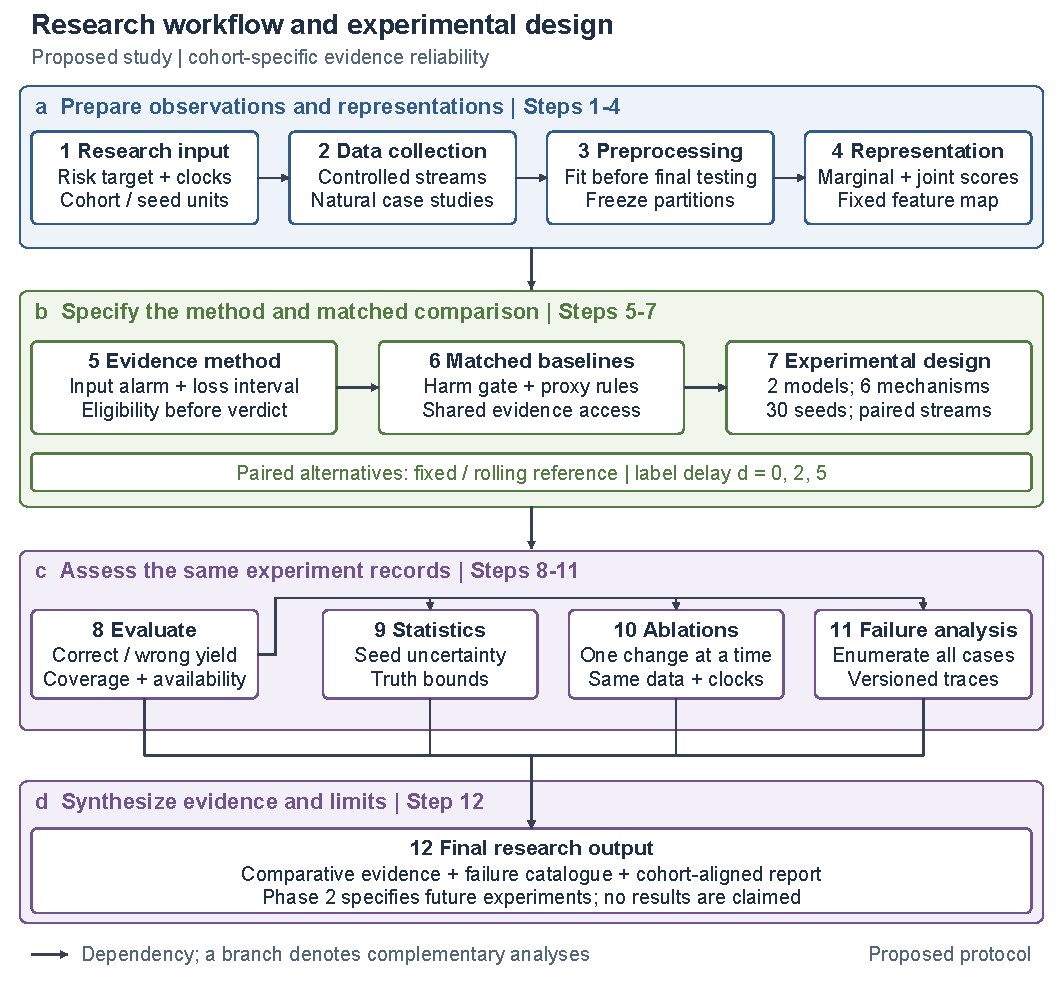
\includegraphics[width=\linewidth]{methodology_overview.pdf}
\caption{Proposed twelve-step research workflow. Preparation (Steps~1--4) feeds
method and experimental specification (Steps~5--7), complementary evaluation
and analysis (Steps~8--11), and research synthesis (Step~12). Reference and delay
alternatives are experimental settings rather than sequential operations.}
\label{fig:overview}
\end{figure}

\begin{figure}[p]
\centering
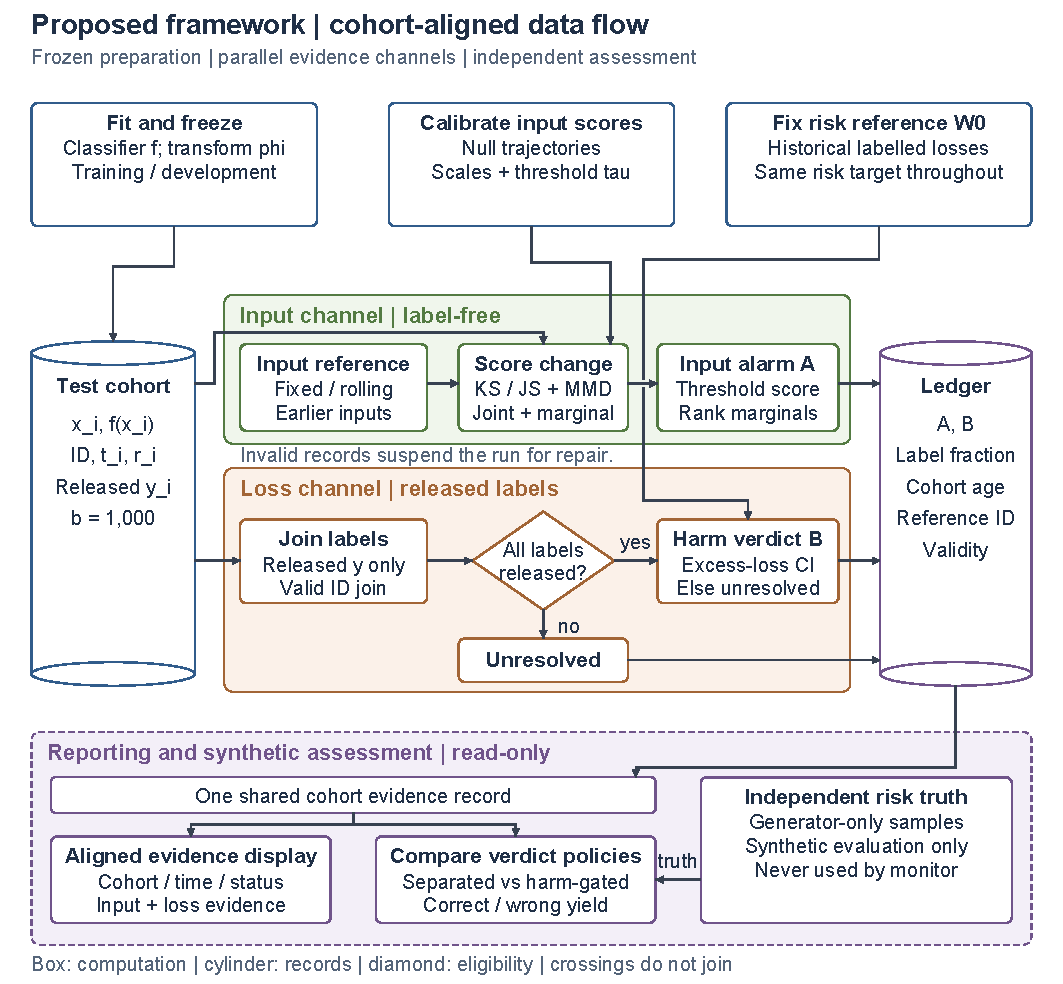
\includegraphics[width=\linewidth]{proposed_framework_architecture.pdf}
\caption{Proposed cohort-aligned evidence architecture. Frozen classifier $f$,
transform $\phi$, input threshold $\tau$ and historical risk reference $W_0$
support two evidence lanes. $A$ denotes the input alarm; $B$ is the interval
verdict after valid joins and complete label release. Input and label-release
times are $t_i,r_i$. Missing labels defer a verdict; invalid records suspend the
run for repair. The common ledger supplies display and policy assessment;
synthetic risk truth reaches the evaluator only. Crossing arrows without a
junction do not join. Natural-data intervals remain exploratory.}
\label{fig:architecture}
\end{figure}

\clearpage
\renewcommand{\refname}{Academic References}
\begin{thebibliography}{99}
\small
\setlength{\itemsep}{3pt}
\bibitem{greco} S. Greco, B. Vacchetti, D. Apiletti, and T. Cerquitelli, ``Unsupervised concept drift detection from deep learning representations in real-time,'' \emph{IEEE Trans. Knowl. Data Eng.}, vol.~37, no.~10, pp.~6232--6245, 2025, doi:~\href{https://doi.org/10.1109/TKDE.2025.3593123}{\nolinkurl{10.1109/TKDE.2025.3593123}}. Reviewed author version: arXiv:2406.17813v2.
\bibitem{szucs} G. Sz\H{u}cs and M. N\'emeth, ``Domino drift effect approach for probability estimation of feature drift in high-dimensional data,'' \emph{Knowl. Inf. Syst.}, vol.~67, no.~5, pp.~4597--4621, 2025, doi:~\href{https://doi.org/10.1007/s10115-025-02362-0}{\nolinkurl{10.1007/s10115-025-02362-0}}.
\bibitem{guerrero} J. V. Guerrero Cano, G. J. Aguiar, and A. Cano, ``Anticipating to change: A proactive approach for concept drift adaptation in data streams,'' \emph{Mach. Learn.}, vol.~115, no.~1, Art.~no.~3, 2026; published online Dec.~14, 2025, doi:~\href{https://doi.org/10.1007/s10994-025-06945-4}{\nolinkurl{10.1007/s10994-025-06945-4}}.
\bibitem{driftvis} W. Yang, Z. Li, M. Liu, Y. Lu, K. Cao, R. Maciejewski, and S. Liu, ``Diagnosing concept drift with visual analytics,'' in \emph{Proc. IEEE Conf. Visual Analytics Sci. Technol. (VAST)}, 2020, pp.~12--23, doi:~\href{https://doi.org/10.1109/VAST50239.2020.00007}{\nolinkurl{10.1109/VAST50239.2020.00007}}.
\bibitem{souza} V. M. A. Souza, D. M. dos Reis, A. G. Maletzke, and G. E. A. P. A. Batista, ``Challenges in benchmarking stream learning algorithms with real-world data,'' \emph{Data Min. Knowl. Discov.}, vol.~34, no.~6, pp.~1805--1858, 2020, doi:~\href{https://doi.org/10.1007/s10618-020-00698-5}{\nolinkurl{10.1007/s10618-020-00698-5}}.
\bibitem{cerqueira} V. Cerqueira, H. M. Gomes, M. Heyden, B. Pfahringer, and A. Bifet, ``A framework for evaluating and benchmarking concept drift detection methods,'' in \emph{Proc. 32nd ACM SIGKDD Conf. Knowl. Discovery Data Mining V.2}, 2026, pp.~8671--8682, doi:~\href{https://doi.org/10.1145/3770855.3819070}{\nolinkurl{10.1145/3770855.3819070}}. Reviewed author version: arXiv:2606.07789v1. \textbf{[Selected study S1]}
\bibitem{window} B. Gower-Winter, M. Groen, and G. Krempl, ``The window dilemma: Why concept drift detection is ill-posed,'' in \emph{Advances in Intelligent Data Analysis XXIV}, LNCS, vol.~16513. Cham, Switzerland: Springer, 2026, pp.~371--384, doi:~\href{https://doi.org/10.1007/978-3-032-23833-7_27}{\nolinkurl{10.1007/978-3-032-23833-7_27}}. Reviewed author version: arXiv:2602.06456v1. \textbf{[Selected study S2]}
\bibitem{pudd} P. Lu, J. Lu, A. Liu, and G. Zhang, ``Early concept drift detection via prediction uncertainty,'' in \emph{Proc. AAAI Conf. Artif. Intell.}, vol.~39, no.~18, 2025, pp.~19124--19132, doi:~\href{https://doi.org/10.1609/aaai.v39i18.34105}{\nolinkurl{10.1609/aaai.v39i18.34105}}. \textbf{[Selected study S3]}
\bibitem{batched} N. Tan, Y.-C. Shih, D. Yang, and A. Salunkhe, ``Flexible and efficient drift detection without labels,'' in \emph{Proc. IEEE Int. Conf. Data Mining Workshops}, 2025, pp.~265--274, doi:~\href{https://doi.org/10.1109/ICDMW69685.2025.00037}{\nolinkurl{10.1109/ICDMW69685.2025.00037}}. Reviewed author version: arXiv:2506.08734v2. \textbf{[Selected study S4]}
\bibitem{causal} D. Komnick, K. Lammers, B. Hammer, V. Vaquet, and F. Hinder, ``Causal explanation of concept drift---A truly actionable approach,'' in \emph{Machine Learning and Principles and Practice of Knowledge Discovery in Databases: ECML PKDD 2025 Workshops}, CCIS, vol.~2842. Cham, Switzerland: Springer, 2026, pp.~396--412, doi:~\href{https://doi.org/10.1007/978-3-032-19105-2_28}{\nolinkurl{10.1007/978-3-032-19105-2_28}}. \textbf{[Selected study S5]}
\bibitem{prodem} A. Sethi, P. Gupta, S. Kansotia, K. Kant, and N. Srivasatava, ``Proactive detection of model degradation in financial fraud prediction with delayed labels,'' in \emph{Machine Learning and Knowledge Discovery in Databases. Applied Data Science Track}, LNAI, vol.~16021. Cham, Switzerland: Springer, 2026, pp.~265--281, doi:~\href{https://doi.org/10.1007/978-3-032-06118-8_16}{\nolinkurl{10.1007/978-3-032-06118-8_16}}. First published online Sep.~29, 2025. Reviewed conference-hosted author version: \url{https://ecmlpkdd-storage.s3.eu-central-1.amazonaws.com/preprints/2025/ads/preprint_ecml_pkdd_2025_ads_315.pdf}. \textbf{[Selected study S6]}
\bibitem{conformal} C. Eliades and H. Papadopoulos, ``A conformal martingales approach for recurrent concept drift,'' in \emph{Proc. 14th Symp. Conformal and Probabilistic Prediction with Applications (COPA)}, PMLR, vol.~266, 2025, pp.~706--724. [Online]. Available: \url{https://proceedings.mlr.press/v266/eliades25a.html}. \textbf{[Selected study S7]}
\bibitem{timans} A. Timans, R. Verma, E. Nalisnick, and C. A. Naesseth, ``On continuous monitoring of risk violations under unknown shift,'' in \emph{Proc. 41st Conf. Uncertainty in Artificial Intelligence (UAI)}, PMLR, vol.~286, 2025, pp.~4204--4226. [Online]. Available: \url{https://proceedings.mlr.press/v286/timans25a.html}. \textbf{[Selected study S8]}
\bibitem{pprm} G. Zhang, Y. Cai, G. Yu, and O. Simeone, ``Prediction-powered risk monitoring of deployed models for detecting harmful distribution shifts,'' in \emph{Proc. 43rd Int. Conf. Machine Learning (ICML)}, PMLR, vol.~306, 2026, pp.~154241--154262. [Online]. Available: \url{https://proceedings.mlr.press/v306/zhang26g.html}. \textbf{[Selected study S9]}
\bibitem{suitability} A. Pouget, M. Yaghini, S. Rabanser, and N. Papernot, ``Suitability filter: A statistical framework for classifier evaluation in real-world deployment settings,'' in \emph{Proc. 42nd Int. Conf. Machine Learning (ICML)}, PMLR, vol.~267, 2025, pp.~49603--49627. [Online]. Available: \url{https://proceedings.mlr.press/v267/pouget25a.html}. \textbf{[Selected study S10]}
\bibitem{navaldata} A. Coraddu, L. Oneto, A. Ghio, S. Savio, D. Anguita, and M. Figari, ``Condition based maintenance of naval propulsion plants,'' UCI Machine Learning Repository, 2014, dataset, doi:~\href{https://doi.org/10.24432/C5K31K}{\nolinkurl{10.24432/C5K31K}}. \emph{Supporting dataset provenance; outside S1--S10.}
\bibitem{shapenergy} B. Teixeira, T. Pinto, and Z. Vale, ``Detecting concept drift with SHapley Additive ExPlanations for intelligent model retraining in energy generation forecasting,'' in \emph{Explainable Artificial Intelligence (xAI)}, CCIS, vol.~2577. Cham, Switzerland: Springer, 2026, pp.~156--168, doi:~\href{https://doi.org/10.1007/978-3-032-08324-1_7}{\nolinkurl{10.1007/978-3-032-08324-1_7}}. First published online Oct.~16, 2025. \emph{Supporting explanation/retraining context; outside S1--S10.}
\bibitem{performative} B. Gower-Winter, G. Krempl, S. Dragomiretskiy, T. Jelsma, and A. Siebes, ``Identifying predictions that influence the future: Detecting performative concept drift in data streams,'' in \emph{Proc. AAAI Conf. Artif. Intell.}, vol.~39, no.~11, 2025, pp.~11726--11734, doi:~\href{https://doi.org/10.1609/aaai.v39i11.33276}{\nolinkurl{10.1609/aaai.v39i11.33276}}. \emph{Supporting feedback-identification context; outside S1--S10.}
\bibitem{badea} D. G. Badea, R.-A. Rotaru, R. V. Rughinis, F. Zaim-Oprea, D. Turcanu, and D. Rosner, ``Detectable, task-relevant, or harmful? Construct-valid evaluation of unlabeled distribution-shift monitoring in chest radiography,'' \emph{J. Imaging}, vol.~12, no.~10, Art.~no.~492, Oct. 2026, doi:~\href{https://doi.org/10.3390/jimaging12100492}{\nolinkurl{10.3390/jimaging12100492}}. \emph{Supporting construct-validity context; outside S1--S10.}
\bibitem{podkopaev} A. Podkopaev and A. Ramdas, ``Tracking the risk of a deployed model and detecting harmful distribution shifts,'' in \emph{Proc. Int. Conf. Learning Representations (ICLR)}, 2022. [Online]. Available: \url{https://openreview.net/forum?id=Ro_zAjZppv}. Reviewed author version: arXiv:2110.06177v4. \emph{Supporting prior work; outside S1--S10.}
\bibitem{solozobov} O. Solozobov, ``Evidence sufficiency under delayed ground truth: Proxy monitoring for risk decision systems,'' arXiv:2604.15740v1, Apr. 2026, preprint. [Online]. Available: \url{https://arxiv.org/abs/2604.15740}. [Accessed: Oct.~26, 2026]. \emph{Supporting prior work; outside S1--S10.}
\bibitem{alencar} B. Alencar, G. Cassales, H. M. Gomes, C. Prazeres, T. Rios, A. Bifet, and R. Rios, ``Concept drift detection in delayed and partially labeled data streams: An experimental survey,'' \emph{Digit. Signal Process.}, vol.~182, Art.~no.~106325, 2026, doi:~\href{https://doi.org/10.1016/j.dsp.2026.106325}{\nolinkurl{10.1016/j.dsp.2026.106325}}.
\bibitem{selective} R. El-Yaniv and Y. Wiener, ``On the foundations of noise-free selective classification,'' \emph{J. Mach. Learn. Res.}, vol.~11, pp.~1605--1641, 2010. [Online]. Available: \url{https://www.jmlr.org/papers/v11/el-yaniv10a.html}.
\bibitem{hoeffding} W. Hoeffding, ``Probability inequalities for sums of bounded random variables,'' \emph{J. Amer. Statist. Assoc.}, vol.~58, no.~301, pp.~13--30, 1963, doi:~\href{https://doi.org/10.1080/01621459.1963.10500830}{\nolinkurl{10.1080/01621459.1963.10500830}}.
\bibitem{nist} E. Tabassi, \emph{Artificial Intelligence Risk Management Framework (AI RMF 1.0)}, Natl. Inst. Standards Technol., Gaithersburg, MD, USA, NIST AI 100-1, Jan. 2023, doi:~\href{https://doi.org/10.6028/NIST.AI.100-1}{\nolinkurl{10.6028/NIST.AI.100-1}}.
\bibitem{awsjoin} Amazon Web Services, ``Ingest Ground Truth labels and merge them with predictions,'' \emph{Amazon SageMaker AI Developer Guide}. [Online]. Available: \url{https://docs.aws.amazon.com/sagemaker/latest/dg/model-monitor-model-quality-merge.html}. [Accessed: Oct.~23, 2026].
\bibitem{gretton} A. Gretton, K. M. Borgwardt, M. J. Rasch, B. Sch\"olkopf, and A. Smola, ``A kernel two-sample test,'' \emph{J. Mach. Learn. Res.}, vol.~13, pp.~723--773, 2012. [Online]. Available: \url{https://www.jmlr.org/papers/v13/gretton12a.html}.
\bibitem{lukats} D. Lukats, O. Zielinski, A. Hahn, and F. Stahl, ``A benchmark and survey of fully unsupervised concept drift detectors on real-world data streams,'' \emph{Int. J. Data Sci. Anal.}, vol.~19, no.~1, pp.~1--31, 2025; first published online Aug.~27, 2024, doi:~\href{https://doi.org/10.1007/s41060-024-00620-y}{\nolinkurl{10.1007/s41060-024-00620-y}}.
\bibitem{kunsch} H. R. K\"unsch, ``The jackknife and the bootstrap for general stationary observations,'' \emph{Ann. Statist.}, vol.~17, no.~3, pp.~1217--1241, 1989, doi:~\href{https://doi.org/10.1214/aos/1176347265}{\nolinkurl{10.1214/aos/1176347265}}.
\bibitem{nistquantiles} Z.-Q. J. Lu, \emph{Estimating Instrument Performance: With Confidence Intervals and Confidence Bounds}, Natl. Inst. Standards Technol., NIST Tech. Note 2119, Sep. 2020, Sec.~5.3, doi:~\href{https://doi.org/10.6028/NIST.TN.2119}{\nolinkurl{10.6028/NIST.TN.2119}}. \emph{Supporting statistical guidance; outside S1--S10.}
\bibitem{awsquality} Amazon Web Services, ``Model quality,'' \emph{Amazon SageMaker AI Developer Guide}. [Online]. Available: \url{https://docs.aws.amazon.com/sagemaker/latest/dg/model-monitor-model-quality.html}. [Accessed: Oct.~23, 2026].
\end{thebibliography}
\end{document}
